\chapter{Deconstructing syntactic theory}

All theories have deep assumptions, i.e. \textit{unknown} unknown knowns. These are the sorts of assumptions which are not questioned, and often cannot be questioned, because they are fundamental to a way of thinking and make an entire program possible. Often we are not aware of such assumptions. Yet by finding and rejecting these very well-hidden assumptions we can make progress toward new, different theories. To do this, we deconstruct the \textit{conceptual metaphors and image schemas}\footnote{There is a substantial literature in cognitive linguistics which formalizes and attempts to regularize notions of conceptual metaphor, image schemas, and blends. The deconstruction pursued here uses these notions informally and in an ad-hoc manner.} that are used to construct conventional syntactic theories. 

  A conceptual metaphor is a set of mappings from a more basic, experientially grounded source domain to a more abstract, conceptual target domain \citep{Lakoff1990,Lakoff1993,Lakoff2008,LakoffJohnson1980a,LakoffJohnson1980b,LakoffJohnson1999,LakoffJohnson200}). An image schema is a pattern generalized over sensory experience (mostly visual), and provides a source domain for conceptual metaphor (\citealt{ClausnerCroft1999,FauconnierTurner1996,FauconnierTurner2008,GibbsColston1995,GradyEtAl1999,Langacker2002,Oakley2007,Talmy1983,Talmy1988};. Theories are constructed by combining, or blending, conceptual metaphors and image schemas \citep{FauconnierTurner1996,FauconnierTurner2008,GradyEtAl1999,LakoffNúñez2000}. The art of theory construction (often a subconscious process) relies on intuitions regarding which metaphors/schemas to blend and which mappings to make use of.

  Many approaches to syntax\footnote{All approaches that I am aware of (present company excluded) are constructed from the delineated metaphors, but there may be other approaches I am not familiar with which are not. I am neither a historian of nor typologist of syntactic theories.}—an in particular generative/minimalist approaches—are constructed from the following set of conceptual metaphors: 

\begin{enumerate}
\item Linguistic units are objects.
\item Linguistic units are containers.
\item Relations between units are connections or containments.
\item Time is space.
\end{enumerate}

  Students of syntax are not taught these metaphors. They do not have to be, because they already know them. Generic versions of these metaphors pervade our conceptual models of abstract domains, and are learned at a fairly early age, especially in literate cultures. Also, there is no point in teaching students these metaphors (if we are even aware of them), because they are not on the table. Teaching them would allow them to be questioned, but they are for the most part non-negotiable. Even being consciously aware of them can be counterproductive, if one wants to participate in the normal discourse. For the lack of a better term, we consider syntactic theories/frameworks which presuppose these metaphors as \textit{conventional}, since it is currently a cultural convention to use these particular metaphors, as opposed to other ones. As mentioned in the introduction, I claim that generative/minimalist theories employ these metaphors, and I encourage the reader to assess their applicability to other theoretical frameworks.

\section{{The} {\textsc{units-}}{\textsc{are}}{\textsc{{}-objects}}{ metaphor}} 

In conventional models, “words” \textit{are} objects. Physical objects, of the sort you can hold. This is a metaphor, a set of mappings from a relatively concrete domain to a more abstract one. The abstract domain is language. The concrete domain is the domain of our experience with physical objects. Via the metaphor, our understanding of words is constructed from aspects of our experience with physical objects. It is not merely the \textit{use} of the word “object” that is crucial here. What is important is that our experience with physical objects is used to reason about metaphorical objects, “words”. For example, our experience with physical objects is such that we can join them together. This physical experience provides a basis for us to think of words as the sorts of things that can be joined together, or \textit{merged}, into larger structures.

  Literally, words are \textit{NOT} objects and are \textit{NOT} merged together in any physical sense. Indeed, “words” are very different from physical objects in many ways. We cannot literally touch words, hold them, join them together, or break them into pieces, etc. Nonetheless, we use the \textsc{words are objects} metaphor to construct a conceptual system for understanding “words”. Crucially, “words” do not exist independently of a conceptual system; rather, a conceptual system gives rise to a concept of a “word”. More generally, in the conventional program, \textsc{linguistic units are objects}: not only words but also phrases, sentences, etc. are objects. A number of mappings are associated with the objects metaphor. To see the importance of these mappings, consider the following descriptions of \textsc{Merge}: 

“The indispensable operation of a recursive system is Merge (or some variant of it), which takes two syntactic \textbf{\textit{objects}} α and β and forms the \textbf{\textit{new object}} γ = \{α, β\}.” \citep[3]{Chomsky2001}.

A natural requirement for efficient computation is a “no-\textbf{tampering} condition” NTC: Merge of X and Y leaves the two SOs \textbf{\textit{unchanged}}. If so, then Merge of X and Y can be taken to yield the set \{X, Y\}, the simplest possibility worth considering. Merge cannot \textbf{\textit{break up}} X or Y, or \textbf{\textit{add new features}} to them. \citep[5-6]{Chomsky2008}.

  Why does \textsc{Merge} “form” a \textit{new} thing? Why is the new thing also an \textit{object}? Why do merged objects not \textit{break up} or have new \textit{features added}? What does it mean for a syntactic object not to be \textit{tampered} with? The proclamations are comprehensible and make intuitive sense because they are consistent with our typical experiences in observing and interacting with physical objects. That is what makes conceptual metaphor so powerful: metaphor allows us to use our experiences with the familiar to construct an understanding of the unfamiliar. 

\subsection{Mappings of the object metaphor}

The conceptual foundations of conventional syntactic theories derive from mapping various aspects of our experiences with physical objects to the abstract domain of syntactic objects. A number of these mappings are catalogued below\footnote{This is neither an exhaustive list nor an essentialist construal of \textit{the} mappings of conventional theories, but rather one possible description of some of the more important ones.} .

  
\begin{figure}
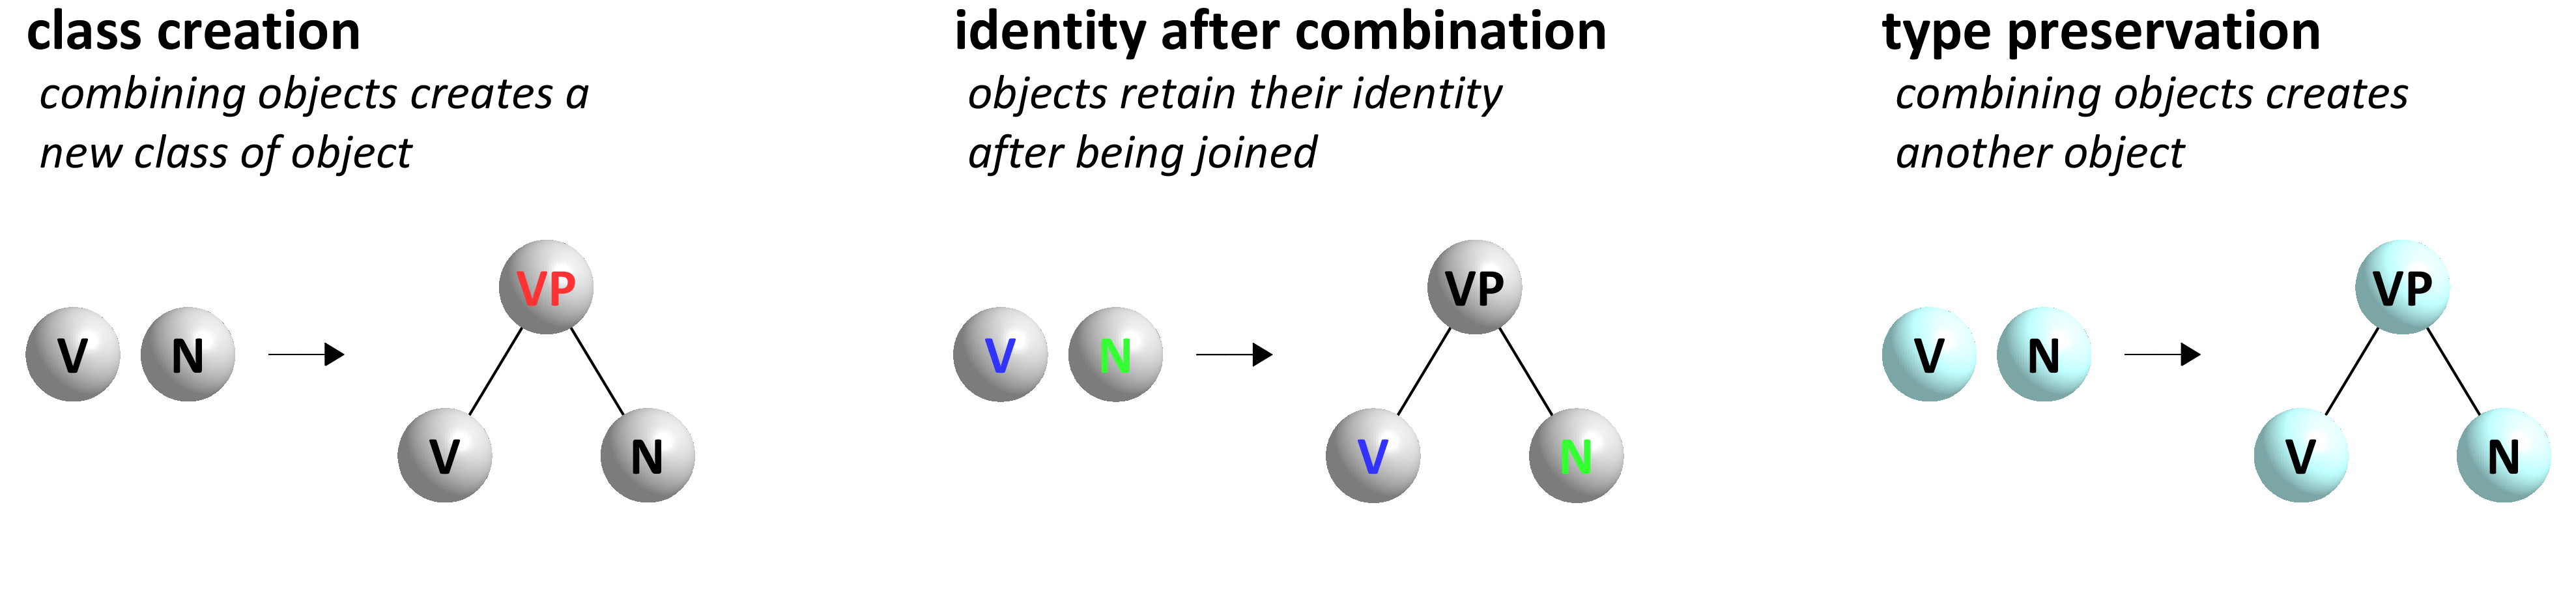
\includegraphics[width=\textwidth]{figures/Tilsen-img29.png}
\caption{Mappings of the object metaphor: class creation, identity after combination, and type preservation.}
\label{fig:3:1}
\end{figure}
 

\textit{Class creation}: combining objects can create a new type of object. When we join a stick and a wedge-shaped stone we “create” an arrow. Likewise, when syntactic objects are combined, a new class of entity is created: word objects are combined to create phrase objects, and phrase objects are combined to create sentence objects. 

\textit{Identity preservation after combination:} the identities of the combined parts are retained after their combination. We can recognize the stick and wedge as continuing to be a stick and wedge after we have joined them, despite the fact that combining them creates a new object, an arrow. Likewise, when syntactic objects are combined, they retain their original identities.

\textit{Preservation of type:} the combination of things of a given type results in another thing of the same type. When we join physical objects, the joined entity is still a physical object. Likewise, the structures which are the inputs of merge are syntactic objects, and the structures which are the output of merge are syntactic objects.

  Mappings of the sort above are profoundly important for theory construction. They are intuitively sensible because they are based on typical experiences, rather than physical principles. Most of the mappings can be violated by considering atypical circumstances (quantum-scale phenomena, far-from-equilibrium chemical reactions, relativistic velocities, etc.). What matters is that in everyday situations, when we join objects together, it creates a new class of object, but we can usually continue to identify the component objects that were joined, and the new class of object is still the same type of thing, i.e. an object. There are many more mappings which come into play, for example:

  
\begin{figure}
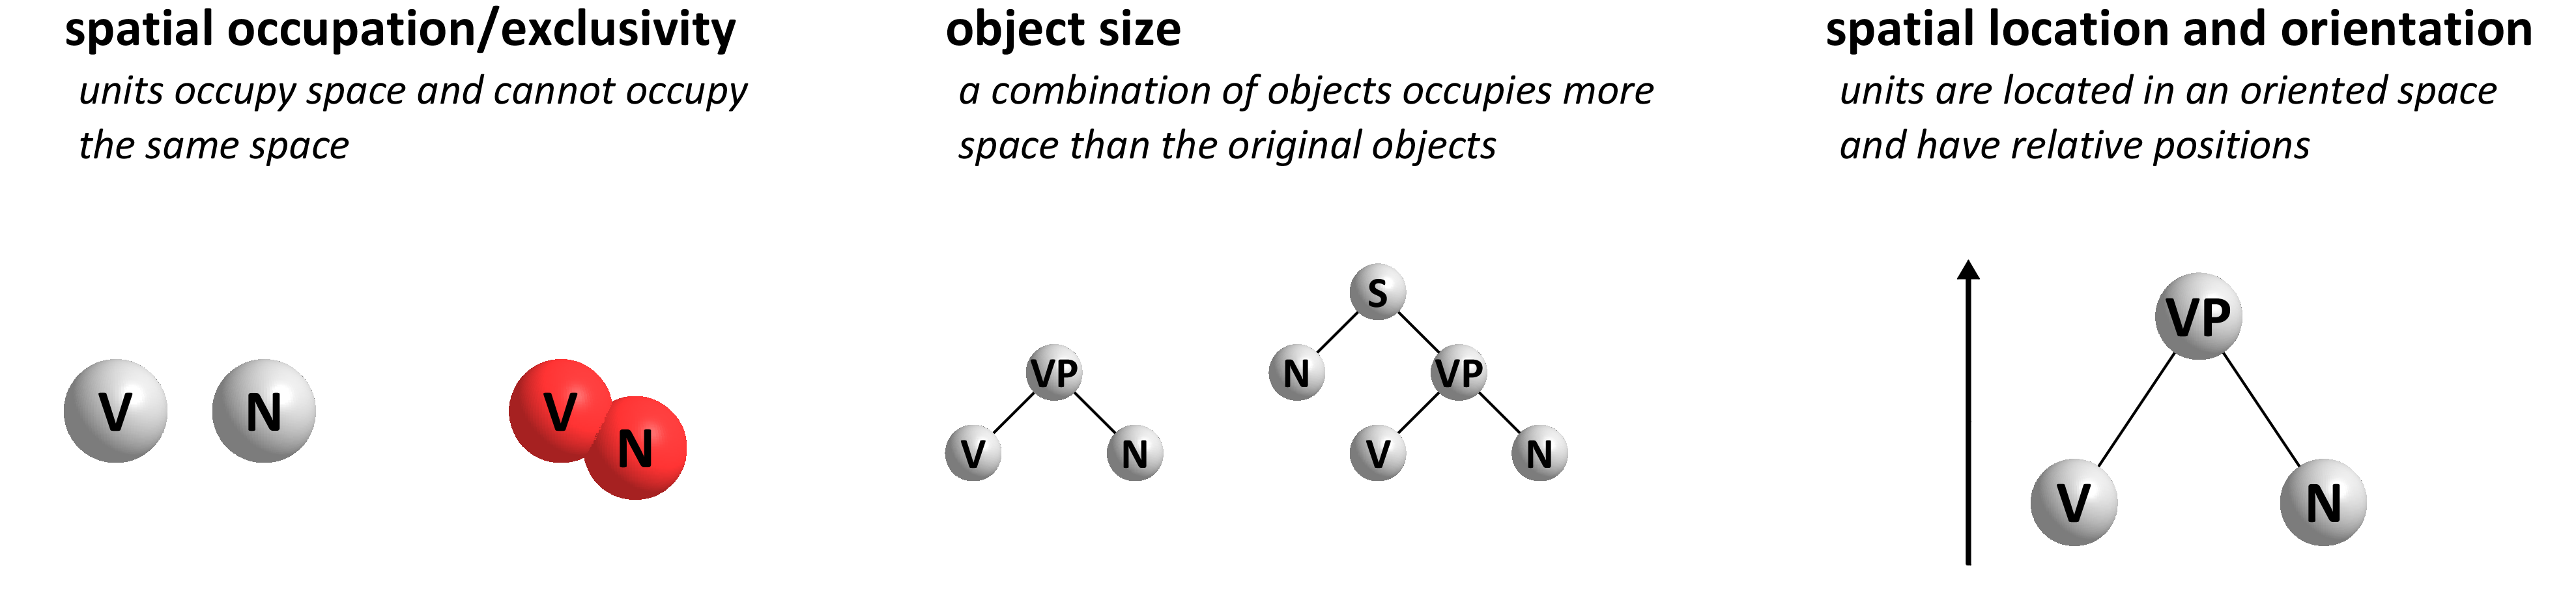
\includegraphics[width=\textwidth]{figures/Tilsen-img30.png}
\caption{Mappings of the object metaphor: spatial occupation, object size, and spatial location and orientation.}
\label{fig:3:2}
\end{figure}
 

\textit{Spatial occupation and exclusivity:} objects occupy space, and spatial occupation is exclusive. My coffee cup takes up some space, and so does my granola bag. Moreover, the coffee cup and granola bag cannot occupy the same space—spatial occupation by objects is mutually exclusive. Likewise, two syntactic objects cannot occupy the same position in a structure. 

\textit{Object size:} when two objects are combined, the combined object occupies more space than either of the original objects. Objects with more parts are larger than objects with fewer parts. Likewise, combining syntactic objects creates a structure that is larger than the original objects.

\textit{Spatial location and orientation}: objects occupy a definite, unique position in an oriented space and have relative locations. The coffee cup and has a definite, unique position in space, and that position can be described relative to the definite, unique position of my granola bag. Likewise, syntactic objects are in definite positions in a structure, and phrases are above the objects which they are composed of.

  
\begin{figure}
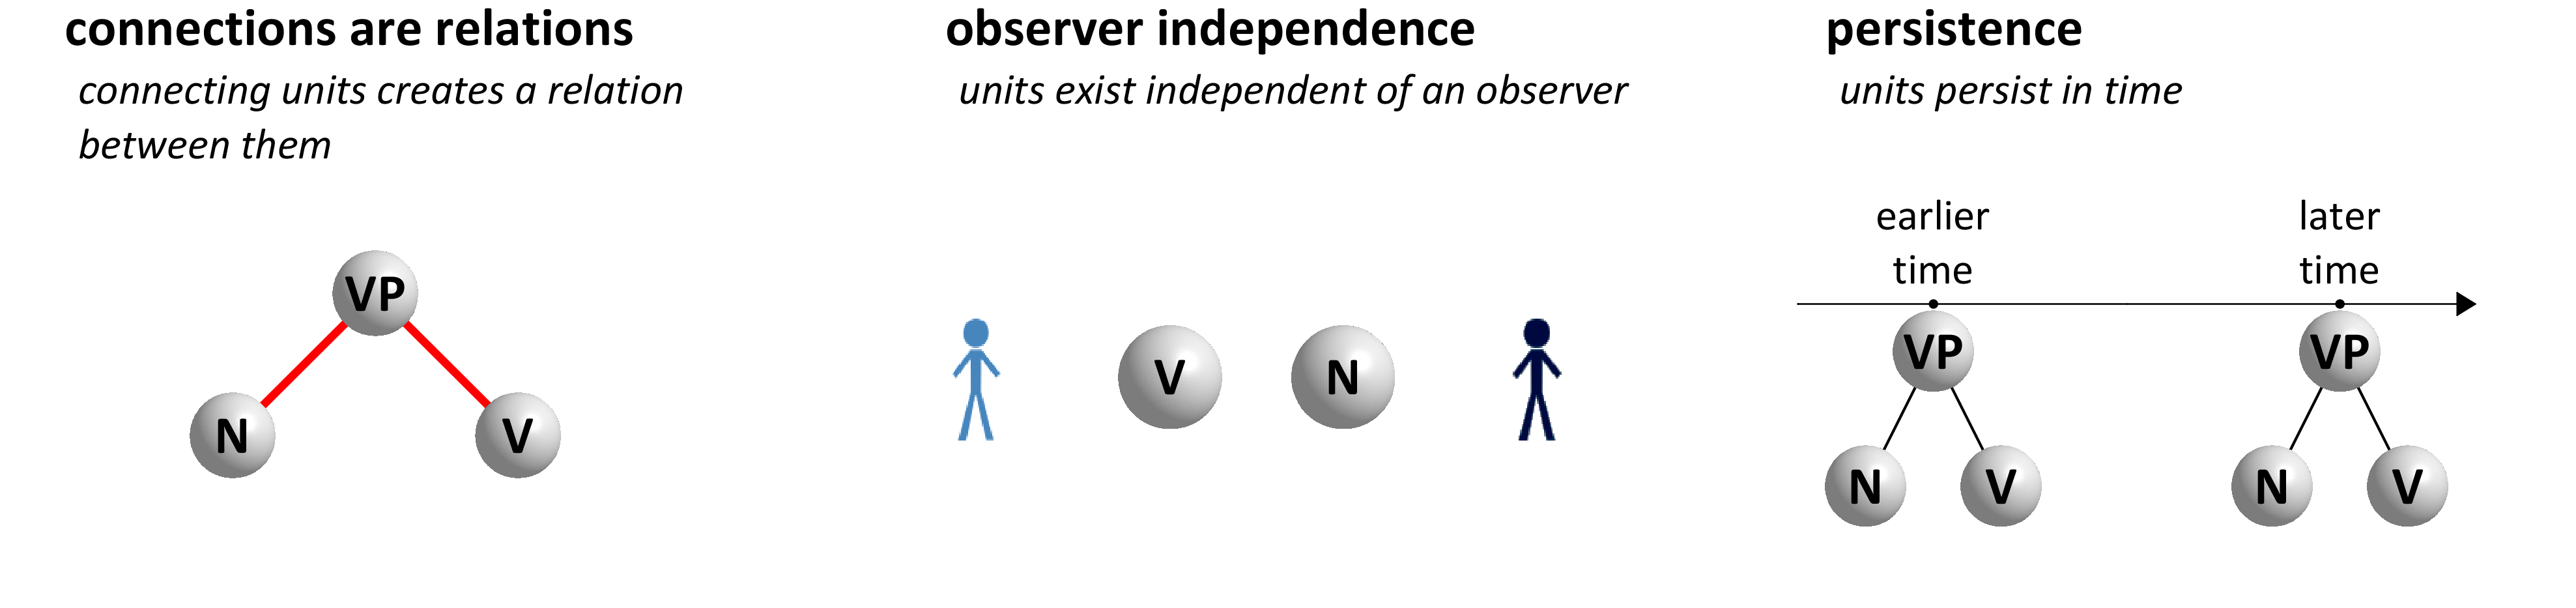
\includegraphics[width=\textwidth]{figures/Tilsen-img31.png}
\caption{Mappings of the object metaphor: connections are relations, observer-independence, temporal persistence.}
\label{fig:3:3}
\end{figure}
 

\textit{Connections are relations:} connecting physical objects creates a relation between them. The pattern of connection often has some functional importance, and constitutes a relation between the connected objects. Likewise, phrases are connected to the units they are composed of.

\textit{Observer-independence:} objects exist and have properties independently of whether they are observed. In our typical experience, the properties of the coffee cup do not depend on who observes or interacts with the cup. Likewise, the properties of syntactic objects do not depend on who speaks or hears them.

\textit{Temporal persistence:} objects persist in time unless acted upon. Our experience tells us that in the absence of other causes, the coffee cup will continue to exist, i.e. the cup will persist in space and in time. Likewise, syntactic structures do not change over time or rearrange themselves in space, unless other mechanisms cause them to.

  The mappings above are just a sample of some of the most fundamental conventional mappings, and more complicated theoretical mechanisms can be understood in terms of them. For example, consider the concepts of movement and traces. In some approaches, the wh-question \textit{What does Al drink}? is formed by first building the structure \textit{Al drinks what} and then by moving \textit{what} and leaving behind a trace, i.e. \textit{What\textsubscript{i} does Al drink} t\textsubscript{i}? The movement is necessary because meaning relations are understood as connections: since \textit{what} has a meaning relation with \textit{drink}, it should be “connected” to \textit{drink}. But the temporal order of words is not consistent with this connection pattern. Meaning relations and word order can lead to conflicting inferences regarding \textit{where} a given unit should be \textit{located} in the structure. This is problematic because an object cannot be in two places at once: the spatial location mapping holds that syntactic objects occupy a unique, definite position, just like the physical objects we are familiar with. To resolve this dilemma, many theories propose to \textit{move} the object, while leaving its original “position” “occupied” by a trace object.

  Hence theoretical devices (e.g. movement and traces) are \textit{consequences} of inferences that follow from the basic metaphors/mappings. Without these mappings, conventional theories would be vastly different. Imagine what conventional theories without identity preservation and temporal persistence would be like: syntactic objects could randomly pop into and out of existence, or morph into other types of objects. Without spatial location, syntactic objects could be in different structural locations at the same time; without spatial occupation/exclusivity, objects could occupy the same position in a structure; without type preservation, we might combine objects to create a substance.

\subsection{The container schema} 

In the conventional paradigm, \textsc{linguistic units are containers}. Words “contain” meanings. Phrases “contain” words. Sentences “contain” phrases. There is meaning \textit{in} my words, there are words \textit{in} phrases, and there are phrases \textit{in} sentences. Descriptions of linguistic structure commonly evoke a container image schema. In its most basic form, the container schema involves a boundary of a region of space. This enables mappings with an inside/outside distinction (cf. \citet{LakoffNúñez2000} for a detailed description of the container schema). Because containers are also objects, containers can be contained. Hence:

“Merge yields the relation \textbf{\textit{Immediately}}{}-\textbf{\textit{Contain}} (IC)…Iterated Merge, required in any recursive system, yields \textbf{\textit{Contain}}. Arguably Merge also yields a relation between α and β (sister)… transitive closure yields C-Command.” \citep[3]{Chomsky2001b}.

  Literally, linguistic units do not physically \textit{contain} meanings or other units. The words \textit{Al}, \textit{drinks}, and \textit{coffee}, are not physically “in” or enclosed within a phrase: one cannot open up a phrase and remove one of the units. There is no physical boundary between the inside and outside of a sentence. Yet we use container-based spatial reasoning pervasively. Below are some mappings which involve the container schema:

  
\begin{figure}
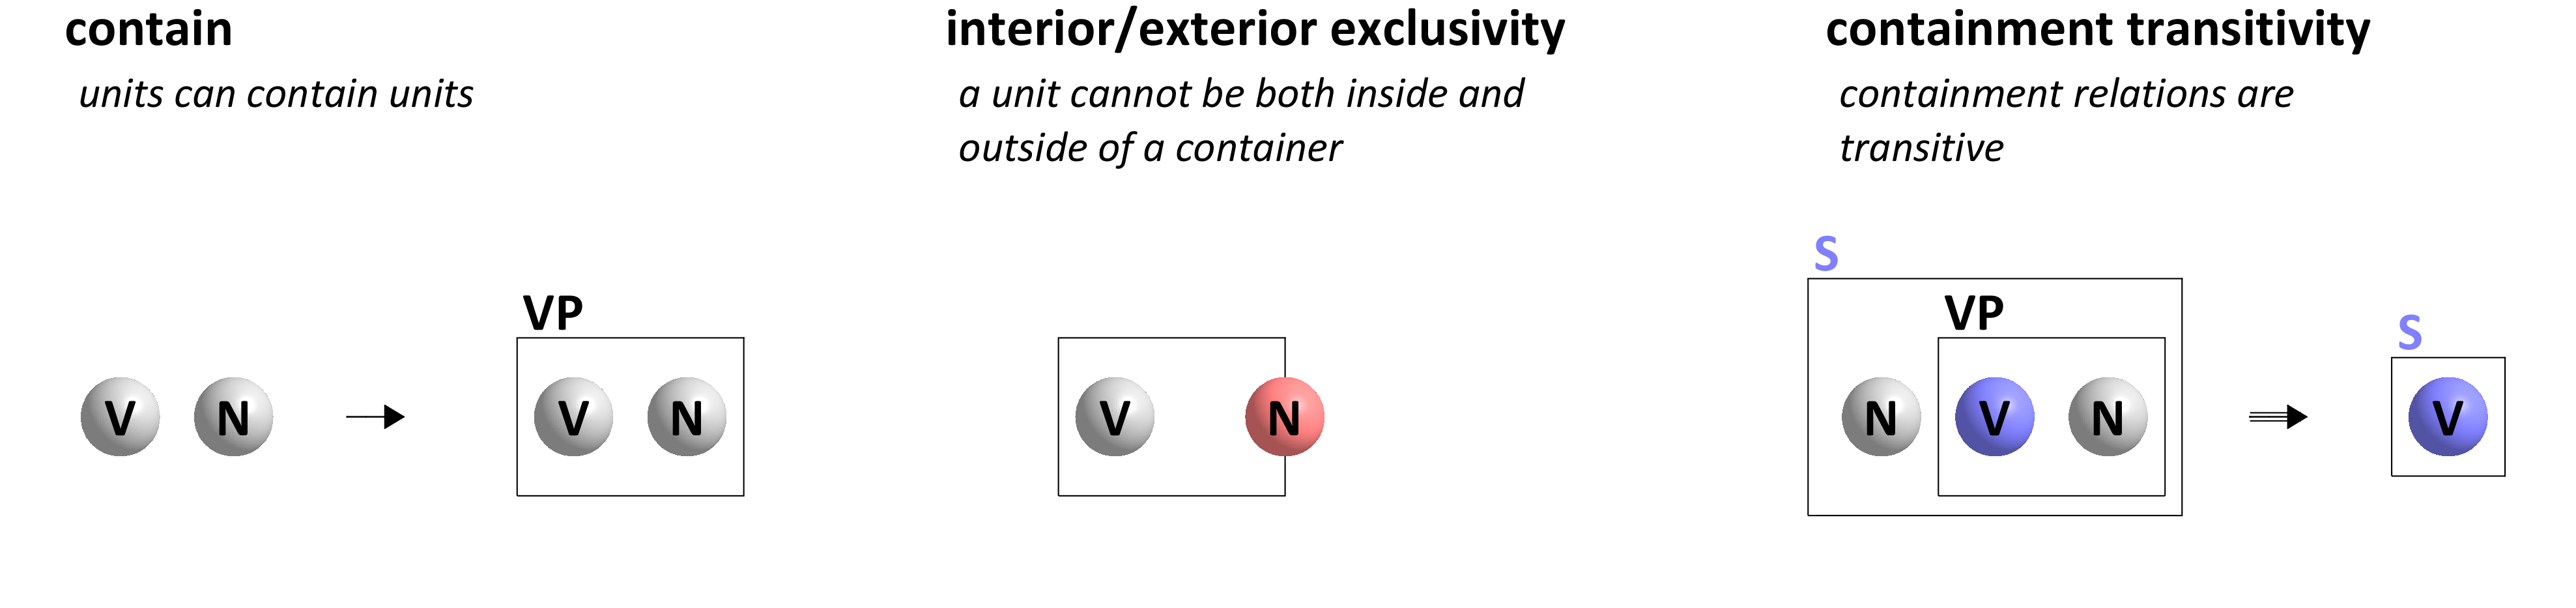
\includegraphics[width=\textwidth]{figures/Tilsen-img32.png}
\caption{Mappings of container schemas: containers can be contained, interior/exterior exclusivity, and transitivity of containment.}
\label{fig:3:4}
\end{figure}
 

\textit{Contain:} containers can be contained. We have plenty of experience with objects being inside an object, which is inside a larger object, etc. My granola is in a bag, the bag is in my backpack, my backpack is in my office, and my office is in a building. Likewise, a linguistic unit can be inside another linguistic unit, which can be inside another linguistic unit, and so on.

\textit{Interior/exterior exclusivity}: an object cannot be both inside and outside of a container. Our typical experience is that objects are either inside or outside of a container. The granola bag is either in my backpack or not; it cannot be both inside and outside of the backpack. Likewise, a linguistic unit is either in a phrase, or not in a phrase, never both.

\textit{Containment transitivity}: if object A contains B, and B contains C, then A contains C. Given that my granola bag is in my backpack, and my backpack is in my office, we can infer via transitivity that the granola bag is in my office. Likewise, if S contains VP, and VP contains V and N, then S contains V and N.

  
\begin{figure}
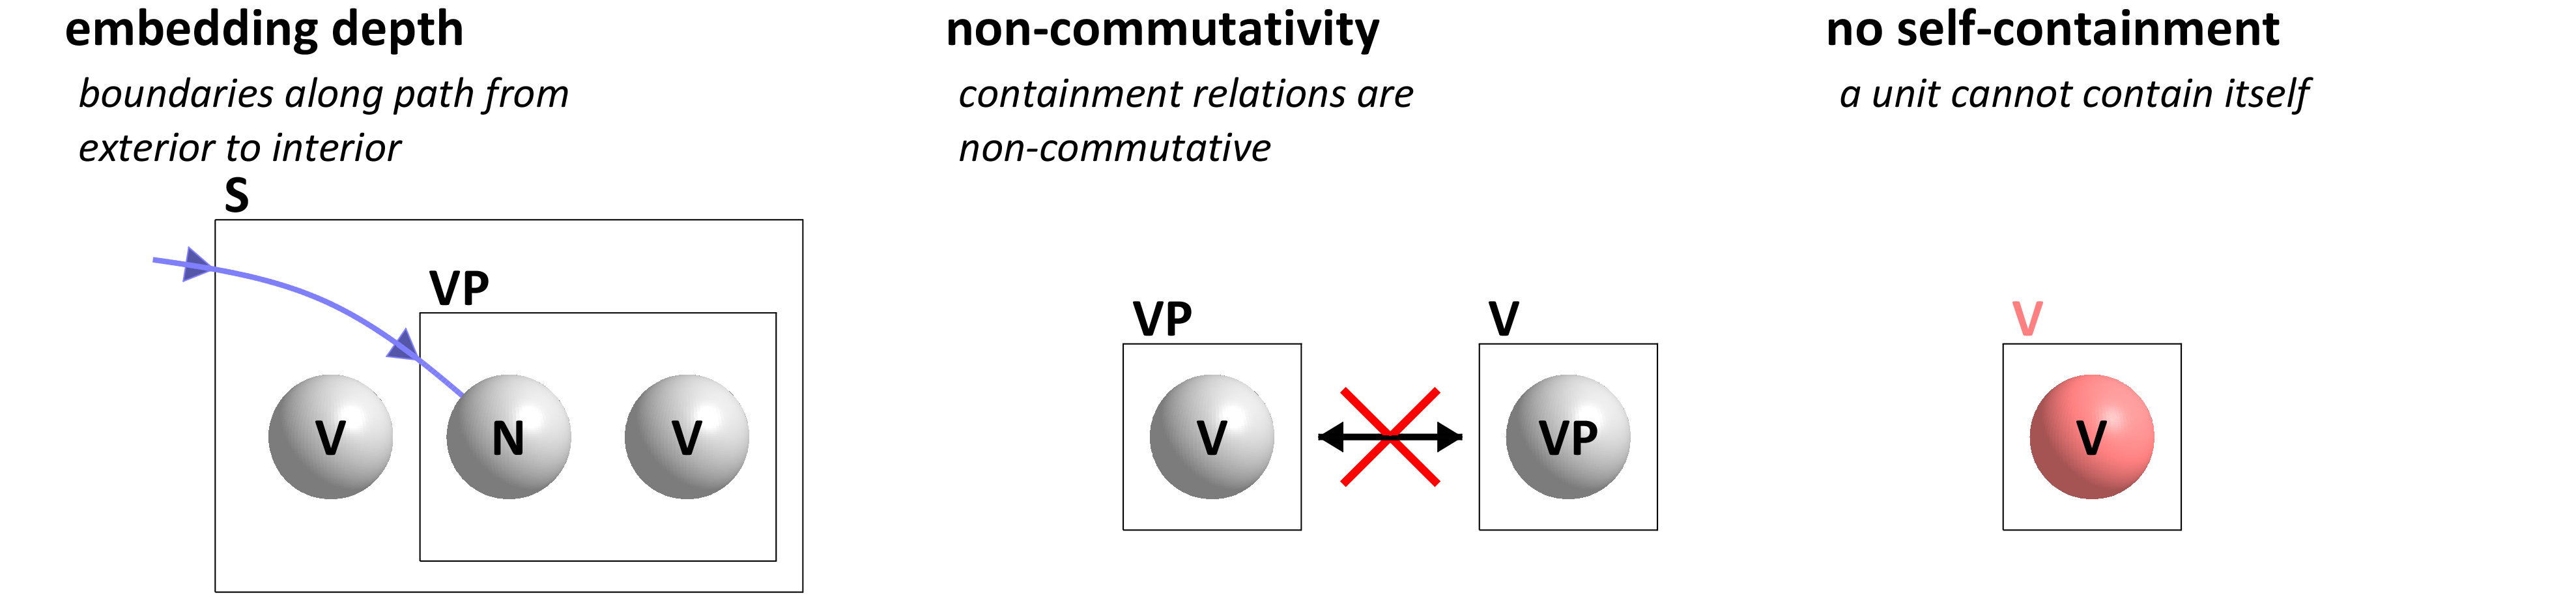
\includegraphics[width=\textwidth]{figures/Tilsen-img33.png}
\caption{Mappings of container schemas: embedding depth, non-commutativity of containment, and prohibition of self-containment.}
\label{fig:3:5}
\end{figure}
 

\textit{Embedding depth}: on a path from the exterior to the interior of a container, the number of boundaries the path crosses is a measure of depth of embedding. From everyday experience, we know that the length of the path can correspond to a number of boundaries encountered. Likewise, the embedding depth of a linguistic unit is measured by a count of containment relations, rather than a distance.

\textit{Non-commutativity}: an object A cannot both contain B and be contained in B. Commutative containment is so far removed from our interactions with physical objects that even imagining it is difficult. Likewise, a linguistic unit can never contain and be contained by the same unit.

\textit{No self-containment}: an object cannot contain itself, either directly or indirectly. We cannot remove an object from itself, nor put an object inside itself. Likewise, a linguistic unit can never contain itself. 

  The above mappings were probably not conscious choices in the construction of conventional theories. They are intuitive consequences of the object metaphor when objects are blended with container schemas. Some of the mappings are so essential to our reasoning that we can hardly imagine a theory without them. Why do linguistic objects never contain themselves? There is no logical necessity for rejecting self-containment, nor an empirical motivation; instead, the avoidance of self-containment of theoretical objects follows from our everyday experience with containment of physical objects. This matters because avoidance of self-containment predetermines how we construct theories. Lets consider once again the motivation for wh-movement. Why not abandon definite, unique spatial location and allow \textit{what} to occupy two positions, i.e. \textit{What}\textsubscript{i does Al drink} (\textit{what}\textsubscript{i})? The answer relates to the connection-containment blend, which we consider next.

\subsection{The connection-containment blend}

A major conceptual divide exists between constituency-based and dependency-based approaches to syntax. Constituency-based (i.e. phrase structure) approaches use a conceptual blend in which relations between units are both patterns of \textit{connection} and patterns of \textit{containment}. This blend allows for structure to be represented with trees (i.e. connected objects) and to also entail containment relations. Dependency-based approaches do not blend containment with connection schemas, and hence do not imply containment relations or phrasal structure (\citealt{Hays1964,Melʹčuk1988,Osborne2006,OsborneEtAl2011,Percival1990,Tesnière2018}). The contrast in schemas is shown below: 

  
\begin{figure}
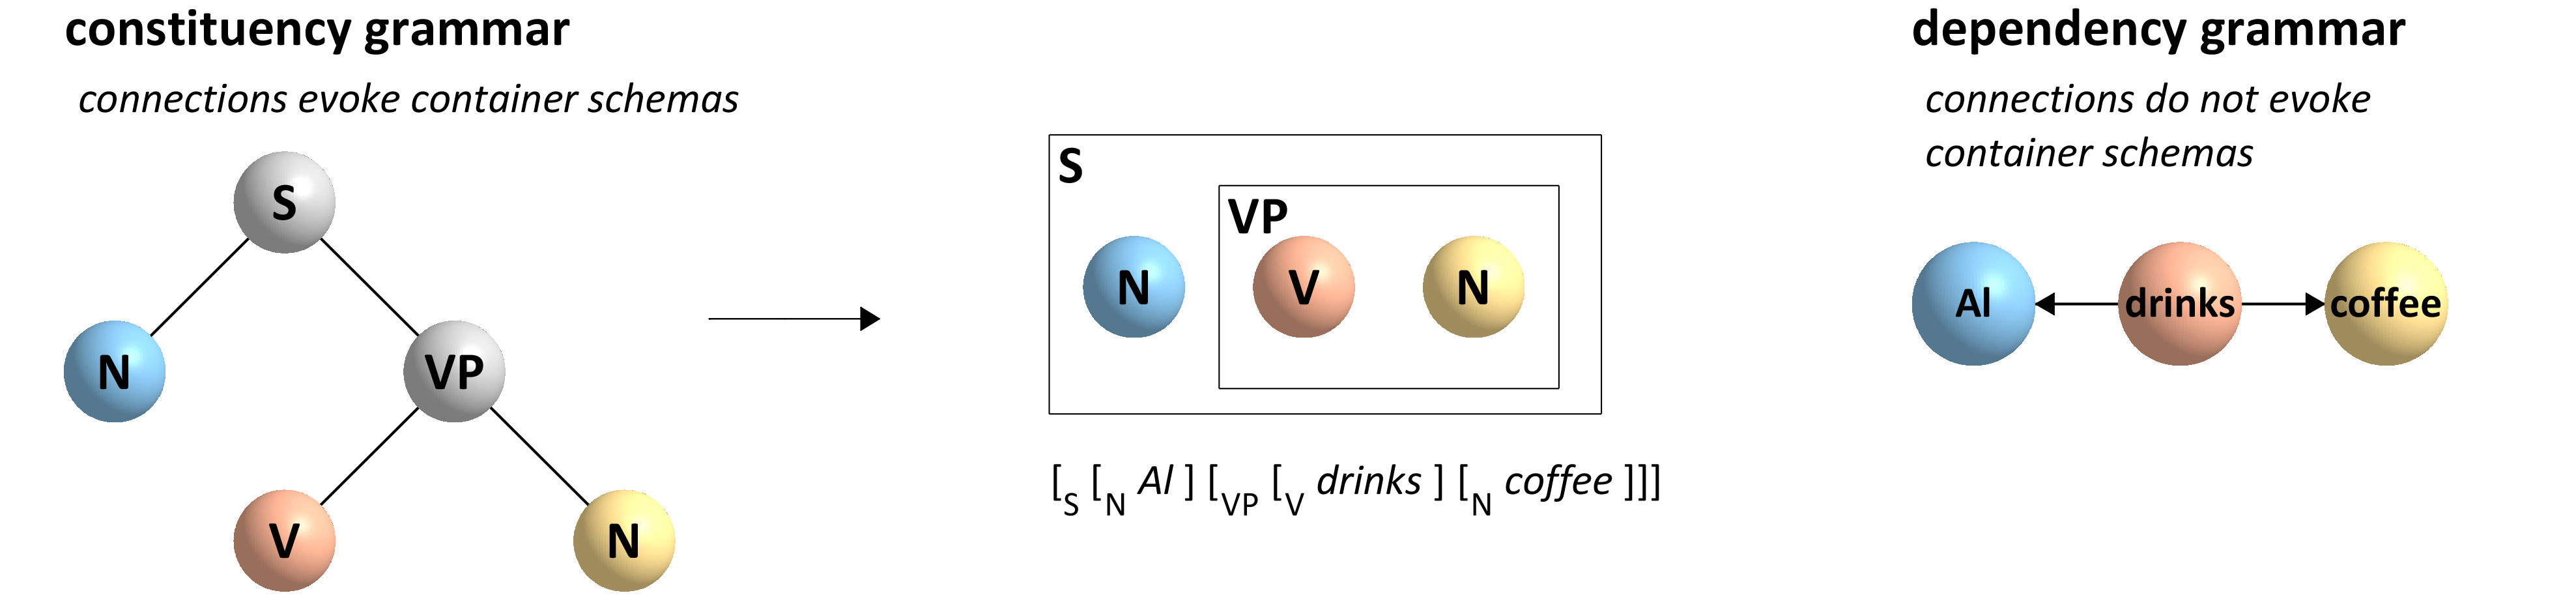
\includegraphics[width=\textwidth]{figures/Tilsen-img34.png}
\caption{Constituency-based models of syntactic structure evoke the connection-containment blend.}
\label{fig:3:6}
\end{figure}
 

  The language used to describe aspects of connection schemas is often mapped from various auxiliary domains, such as trees, families, and networks. Hence a location in a structure where “branches” join is a “node”, an end of a “branch” is a “terminal node”. One unit can “dominate” another, or can be a “parent” or “child”, and can have “siblings”. Dominance and precedence relations can be immediate or non-immediate, depending on whether there are any nodes on the \textit{path} of connections between them. The differences between auxiliary source domains (trees, families, networks, etc.) tend to be superficial and of trivial importance. It is the more abstract and basic schema of connection, and the blending of connection with containment, which is crucial.   

  The conventional construct of a \textit{phrase} relies heavily on a blend of connection and containment schemas. Parent-child connections (i.e. dominance relations) are understood as containment relations. By convention, relational asymmetries in containment are implicit in the relative vertical locations of connected objects, with parent units located \textit{above} child units. For example in (A) below, the object N in the tree structure is \textit{inside} the VP, i.e. is a subconstituent of the VP, but the connection does not overtly show this. Containment must therefore be inferred by convention from relative orientation: N is both connected to VP \textit{and} is lower than VP. The particular direction of the orientational mapping comes from an \textit{up is more} metaphor, but one can readily imagine the reverse. The orientation of (A) is unnecessary if connections are directed, as in (B). We can thus interpret relative vertical orientation as a form of implicit directionality in connections. The orientation information greatly facilitates the containment-connection blend because it is easier to superimpose containment schemas on structures like the one in (A) than the one in (B). 

  
\begin{figure}
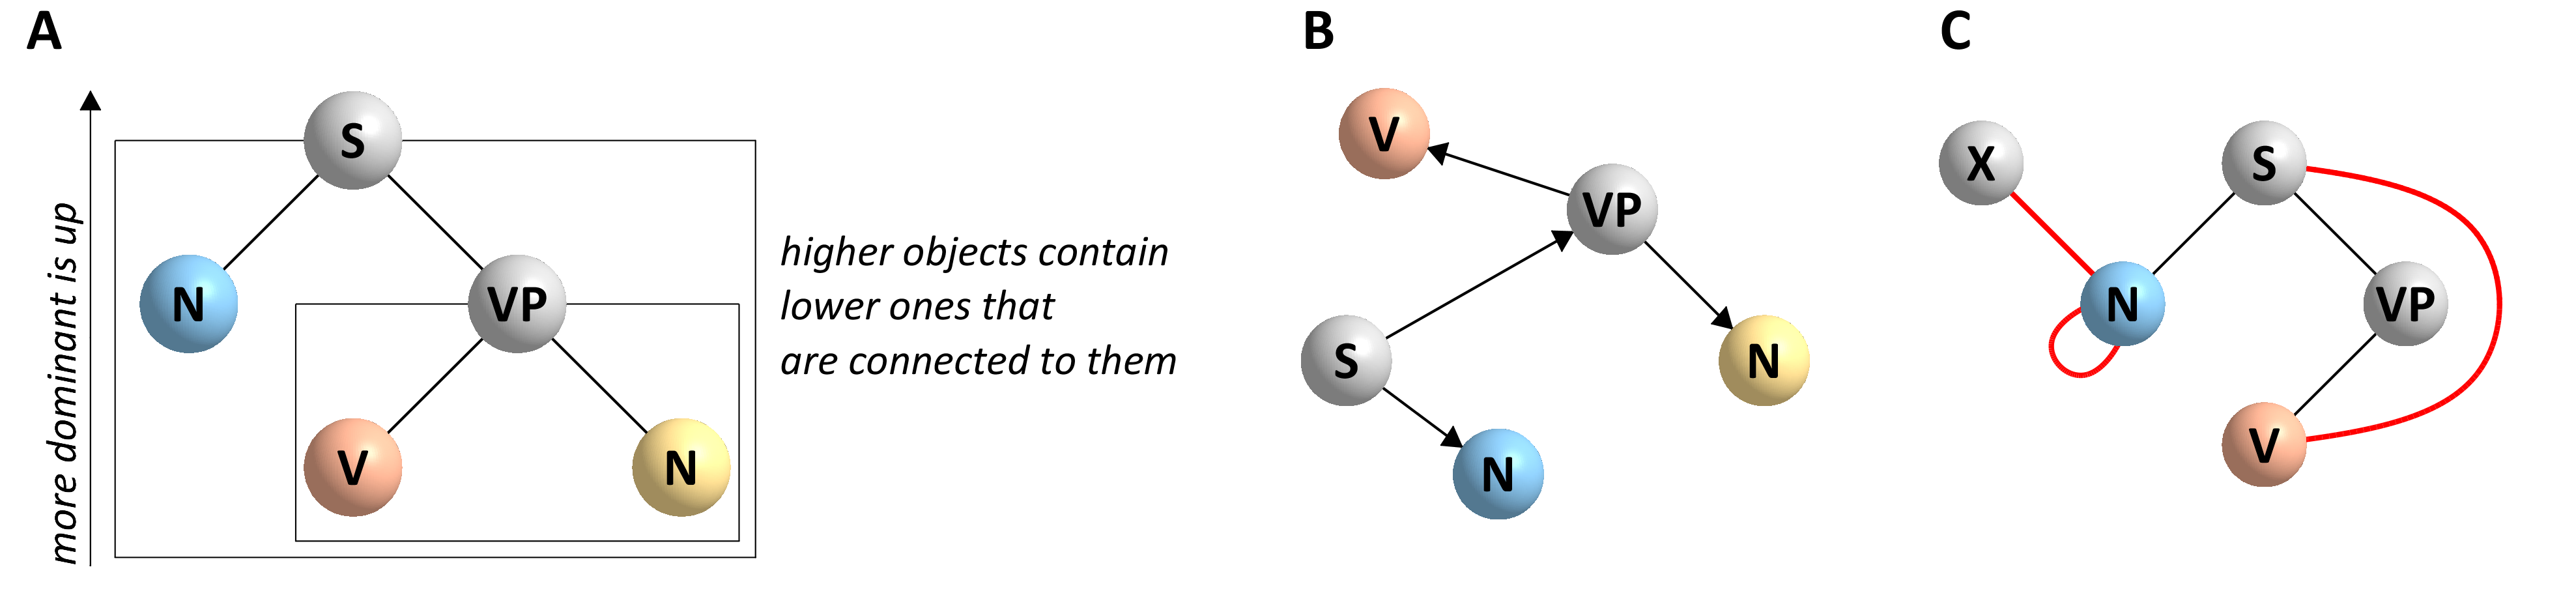
\includegraphics[width=\textwidth]{figures/Tilsen-img35.png}
\caption{The role of vertical orientation in the connection-containment blend.}
\label{fig:3:7}
\end{figure}
 

  The mappings of the connection-containment blend explain why self-connections are disallowed and why a lower unit cannot dominate a higher one. Self-connection as in (C) would imply self-containment, and allowing for lower units to dominate higher ones (i.e. abandoning the implicit orientation/directionality) would lead to indirect self-containment. A node cannot have two parents, i.e. never connects to two nodes above it, because this would lead to ambiguity in which parent container is the most external. If A contains C and B contains C, then to avoid such ambiguity either A contains B or B contains A; but the situation in example (C) where both X and S are connected to N gives rise to an ambiguity in the containment relation between X and S. Crucially, prohibitions on self-connection and multiple parents are not a necessary consequence of using connection schemas; the prohibitions arise from blending connection with containment.

  The connection-containment blend is powerful because it associates connection schemas with additional conceptual structure involving containment, without adding visual clutter to a representation. Note that there is a visual incompatibility between connection and containment, such that simultaneous depictions of connection and containment are problematic if one wishes to avoid connection paths or objects crossing container boundaries, as in (A). The blend is a useful tool because it hides this incompatibility: with just a little practice, we learn to infer containment patterns from connection patterns (and vice versa), without the need to envision both simultaneously. The use of orientation to indicate relational asymmetries makes the blend possible.

\subsection{{\textbf{The contingency of the object metaphor}}}

Why do the object metaphor and connection/containment schemas dominate linguistic theory? Does it have to be this way? Perhaps it is our early experience with the technology of writing. Written words on a page occupy physical space, so it is natural to extend that experience to abstract reasoning about language. Before written language, did humans think of words as objects? Probably not (\citealt{Linell1988,Linell2005,Ong2013}), and so we must see our current conceptual frameworks as accidental, historical contingencies. This calls into question the value of those approaches. On the other hand, perhaps written words are spatially ordered because we have some species-specific cognitive predisposition for spatial order, a predisposition which may derive from our biological architecture. Even so, the object metaphor would still be contingent on evolutionary-scale forces. 

  We \textit{can} consider alternative metaphors. A fairly simple example is the \textit{substance metaphor}, which has mixing-related mappings instead of connection or containment. Lets think of the combination of a noun and a verb as a mixing of substances. Physical mixing often gives rise to a substance with new properties, which may not necessarily be predictable from the component substances; in a sense, the component substances lose their original identities. This seems analogous to the creation of idiomatic verb phrases from verbs and nouns: \textit{bite the dust}, \textit{break a leg}, etc. The point is that other mappings, which derive from other metaphors, could be on the table.

  The metaphors of the o/el framework are very different from the conventional ones, and this creates problems when using conventional terminology. The term “linguistic unit” so strongly evokes the object metaphor and related schemas, that its use is jarring in an o/el context. For example, in the o/el paradigm, we might adopt the metaphor \textsc{linguistic units are trajectories in a state space}. But this is absurd: how can a unit (as object) \textit{be} a trajectory? The cognitive dissonance here reveals just how deeply the tentacles of object metaphor have insinuated our cognitive models of language.

  Remember: there is no such thing as “a linguistic unit”. One must do some hard work to see that “units” are not and cannot be objects; instead, one should loosely associate the conventional construct of a unit with an experience corresponding to a trajectory in a state space. The dimensions of the space are excitation values (e) and phases (θ) of conceptual and syntactic systems. Relations between “units” are associated with particular geometries of trajectories in this state space. Avoiding the term \textit{linguistic unit} altogether is a good idea, because of its propensity to evoke the object metaphor. Thus we prefer to say that \textsc{linguistic patterns are system trajectories in a state space}\footnote{Linguistic patterns are understood metonymically here as the products (behaviors) which result from trajectories in a state space. Ultimately it is better not to reify language: language \textit{IS} nothing, i.e. not a thing: people act and we attempt to understand those actions; language is one of our analytical categories of actions.}.

  The dominance of the object metaphor is a cultural or evolutionary contingency, rather than a necessity. But the use of \textit{some} metaphors, whatever they are, is unavoidable. We need metaphors because the systems we want to understand—those involved in language and cognition—are so very complex, and metaphors are the tools we have for constructing understandings of complex phenomena. We should try to be more aware of which metaphors we choose, and we can choose to explore new metaphors.

\subsection{Object multiplicity}

The conventional mappings of the object metaphor, in particular spatial occupation and temporal persistence, necessitate co-presence and therefore \textit{object multiplicity}. Syntactic objects are \textit{present} in a space. What does it mean for objects “to be present” “in” a “space”? Via spatial occupation and persistence mappings, the object metaphor entails that all of the objects in a structure are \textit{there}, i.e. co-present in some space at some time. Hence for many utterances, a multiplicitous representation is necessary: multiple instantiations of a given type of object are simultaneously present. Consider the utterance shown below, \textit{Dee knows that Cam knows that Bo knows that Al drinks coffee}. The multiplicitous representation in (A) shows many instantiations of each syntactic category, and many copies of the verb \textit{knows}.

  A non-multiplicitous connected object representation as in (B) necessarily violates some mappings of the connection-containment blend. It looks very much like a finite state model (without transition probabilities), which is the very conception that generative grammar originated in reaction to \citep{Chomsky1956}. The structure in (B) violates a number of conventional mappings: containment is not transitive; there is self-containment; relative vertical orientation does not map to containment/dominance; the typical notion of embedding depth is not available. Moreover, a structure of this sort cannot be constructed through \textsc{Merge}: each word must be associated with its own syntactic object; words cannot share the same object. Hence we conclude that multiplicity is a consequence of object co-presence and connection/containment mappings.

  
\begin{figure}
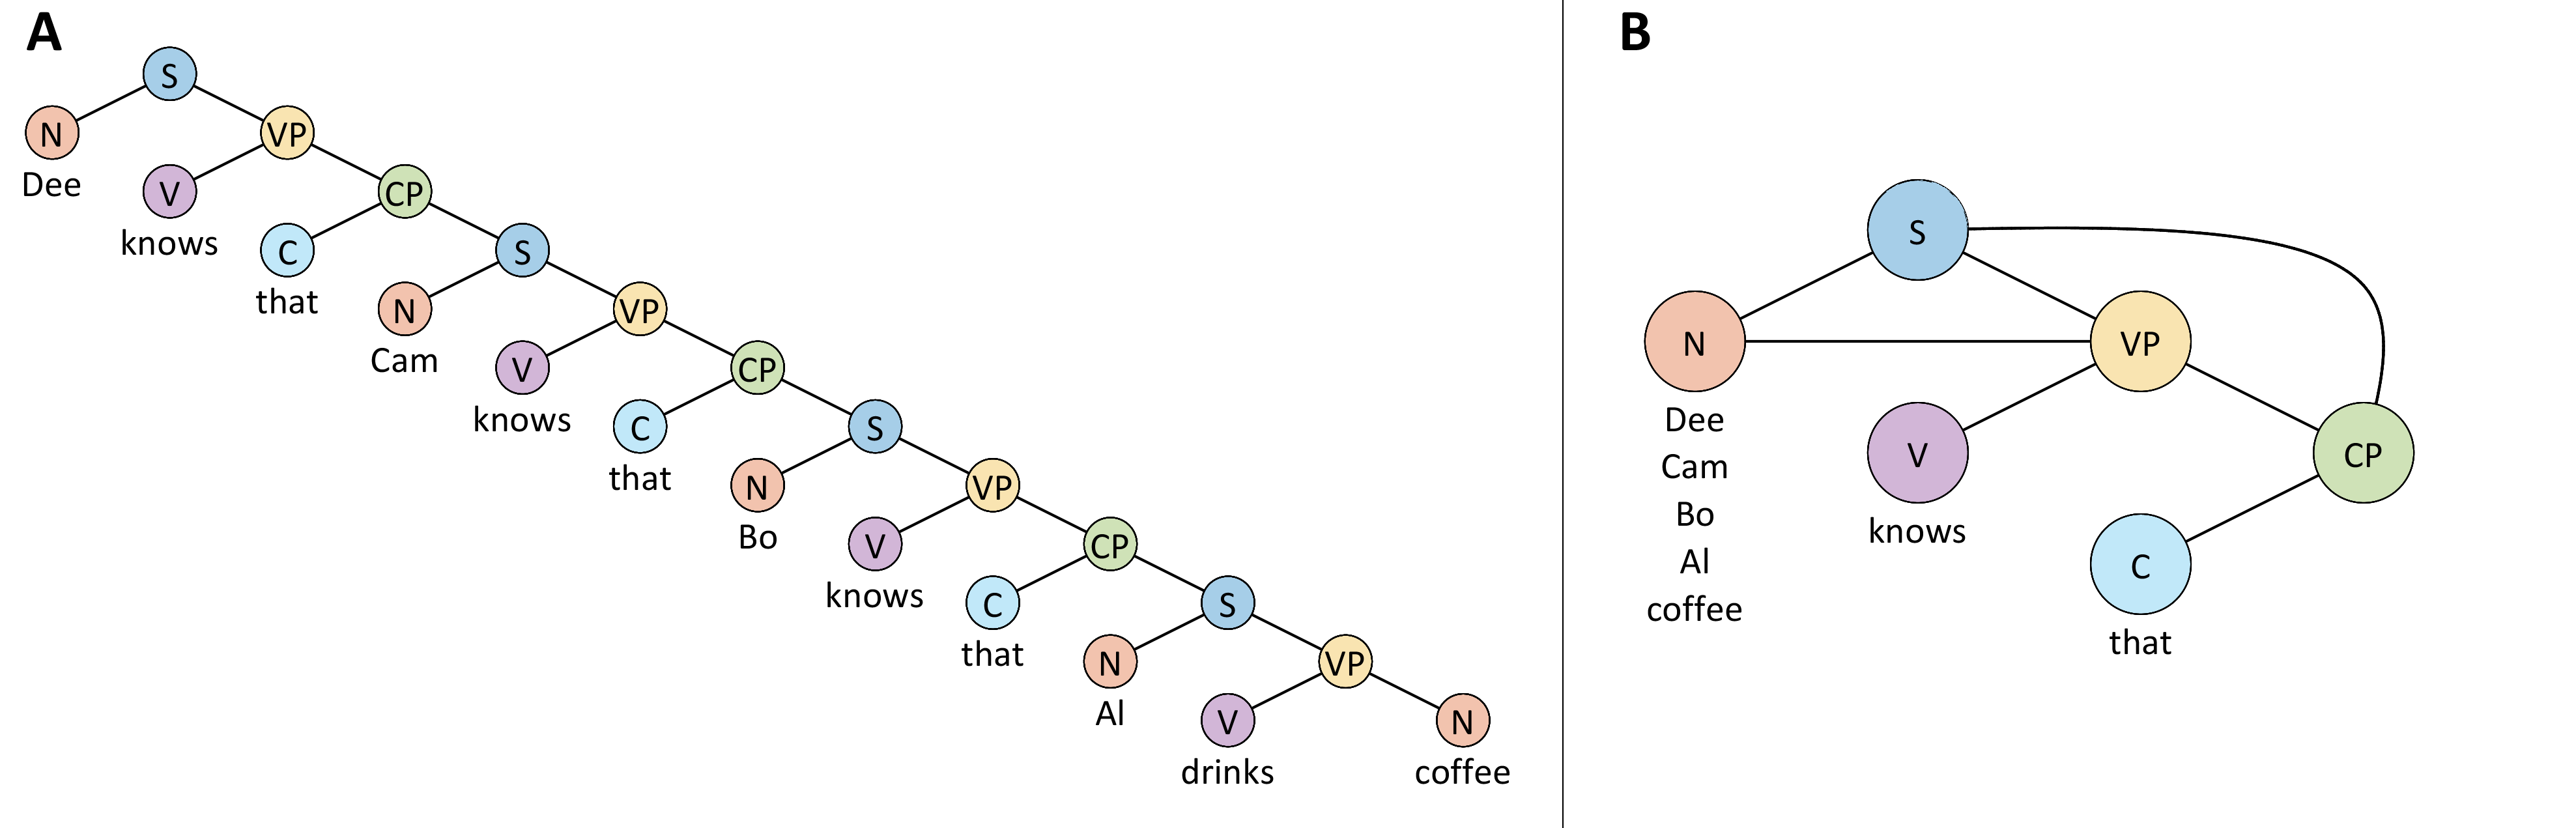
\includegraphics[width=\textwidth]{figures/Tilsen-img36.png}
\caption{The connection-containment blend necessitates multiplicitous representations.}
\label{fig:3:8}
\end{figure}
 

  The problem with multiplicitous representations is that they prevent us from recognizing an important phenomenon: \textit{interference}. In the o/el framework, each concept system resonates with a syntactic system. Both types of systems are, microscopically, neural populations of finite size. In order for two c-systems such as [Al] and [Bo] to simultaneously resonate with the same \{+N\} s-system, the s-system population must \textit{differentiate} into two subpopulations, where each subpopulation interacts more strongly with one or the other of the two concept populations. But this differentiation cannot be perfect: the s-system subpopulations overlap and will interact with one another, and hence the c-systems will interfere with one another, indirectly, via their resonances with the differentiated s-systems. 

  
\begin{figure}
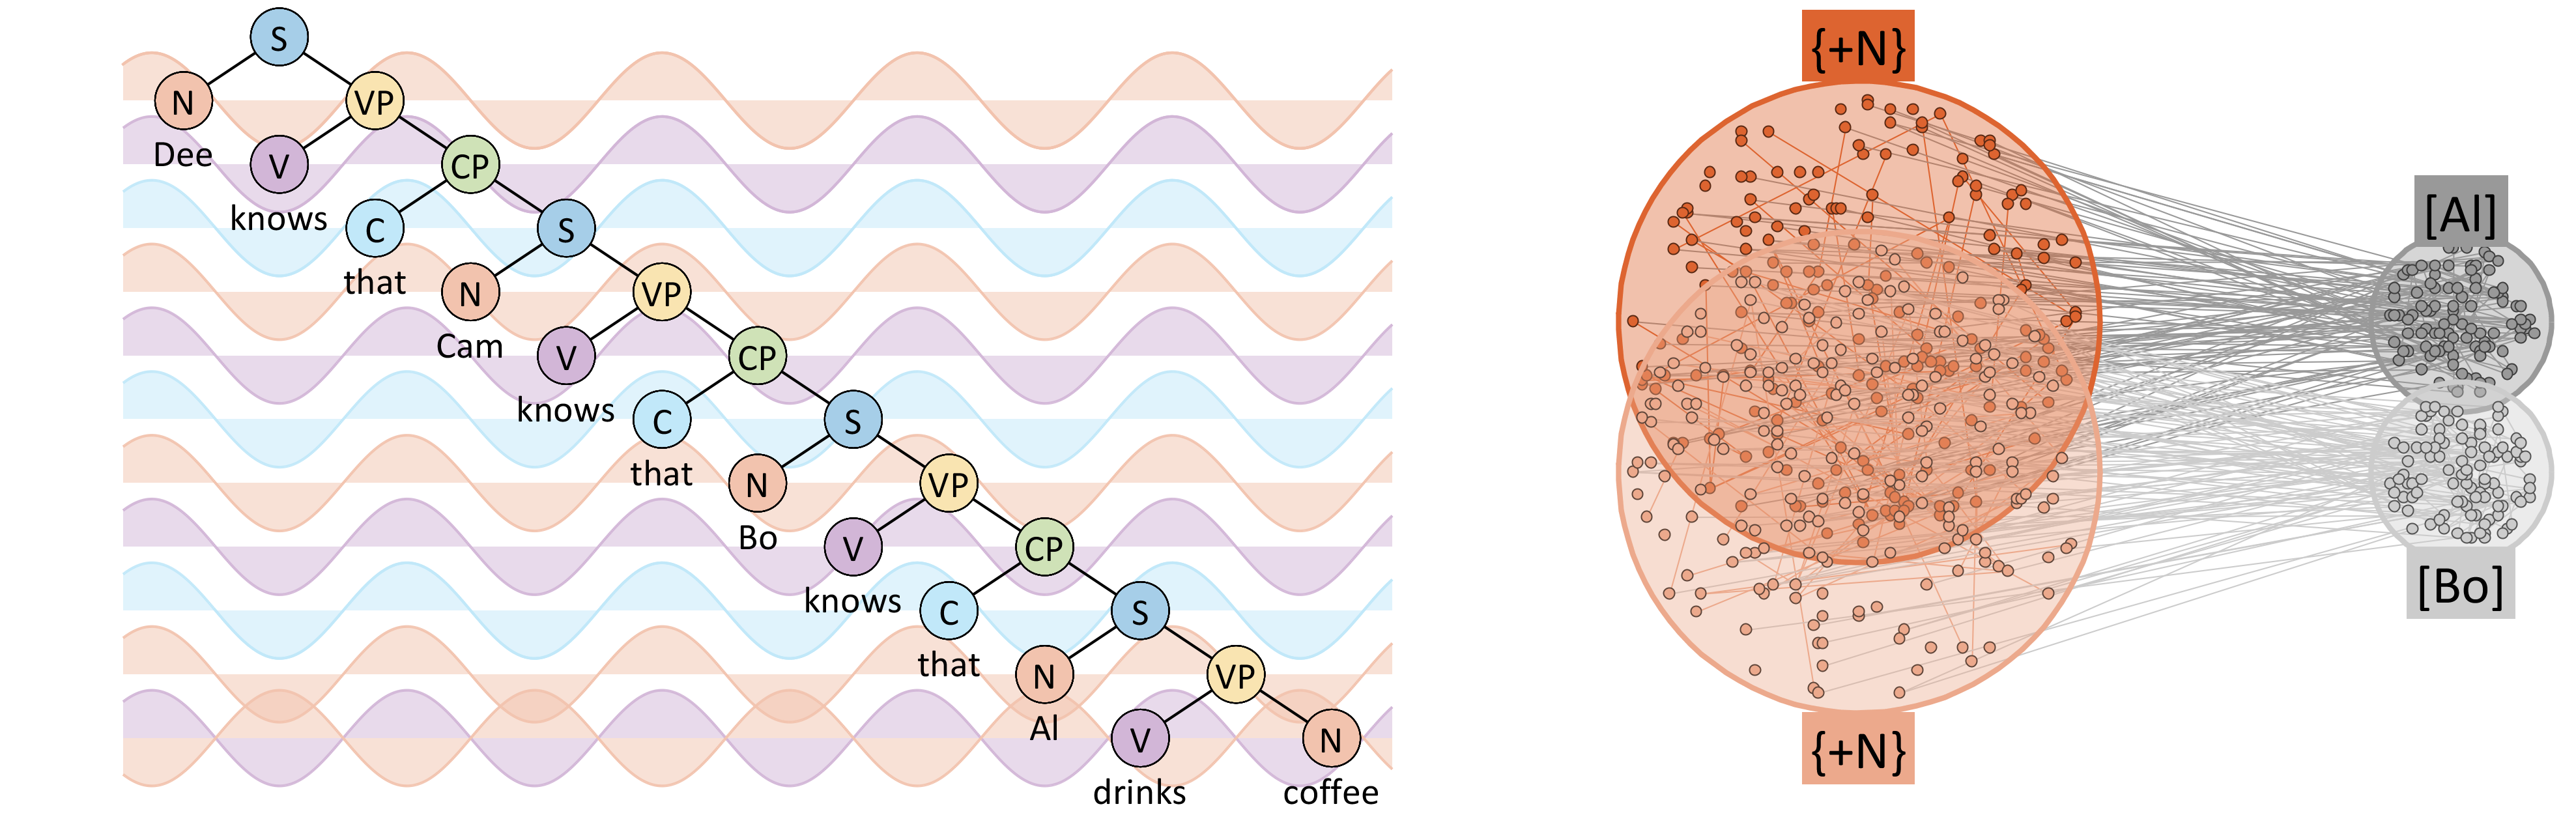
\includegraphics[width=\textwidth]{figures/Tilsen-img37.png}
\caption{Two c-systems which simultaneously resonate with an s-system can infere with one another.}
\label{fig:3:9}
\end{figure}
 

  The conventional metaphors give us no reason to expect limitations on the number of “copies” of an object. The object metaphor and connection-containment blend necessitate multiplicity. But the brain, a physical system, cannot work this way. There must be limits on the differentiation of populations, because of their finite sizes. More to the point, the brain cannot create arbitrarily many copies, or even two copies, of the same object, because linguistic units are not \textit{objects} in the first place and thus cannot be copied. In the o/el framework, we see why multiplicity is a problem, and we can explore how interference constrains the organization of syntactic and conceptual systems.

\section{The time-is-space metaphor}

In all human cultures, there are spatial metaphors/image schemas for conceptualizing time. A very general one is the metaphor that \textit{temporal order is spatial order}, or more tersely, \textit{time is space} (\citealt{Boroditsky2000,Boroditsky2001,CasasantoBoroditsky2008,Evans2006,GentnerEtAl2002,LakoffJohnson1999,NúñezEtAl2006}). In the most common variant of the metaphor, time is a \textit{linear} space. Another variant involves a periodic space, where times are locations on a circle, or phase angles. In both of these schemas, there are events and an observer, and there are two different ways in which the observer and events can be mapped to the schema. In one, the observer is moving and events are objects located in the space through which the observer moves. In the other, the observer is stationary and events are moving objects which pass by the observer. These variations are shown below:

  
\begin{figure}
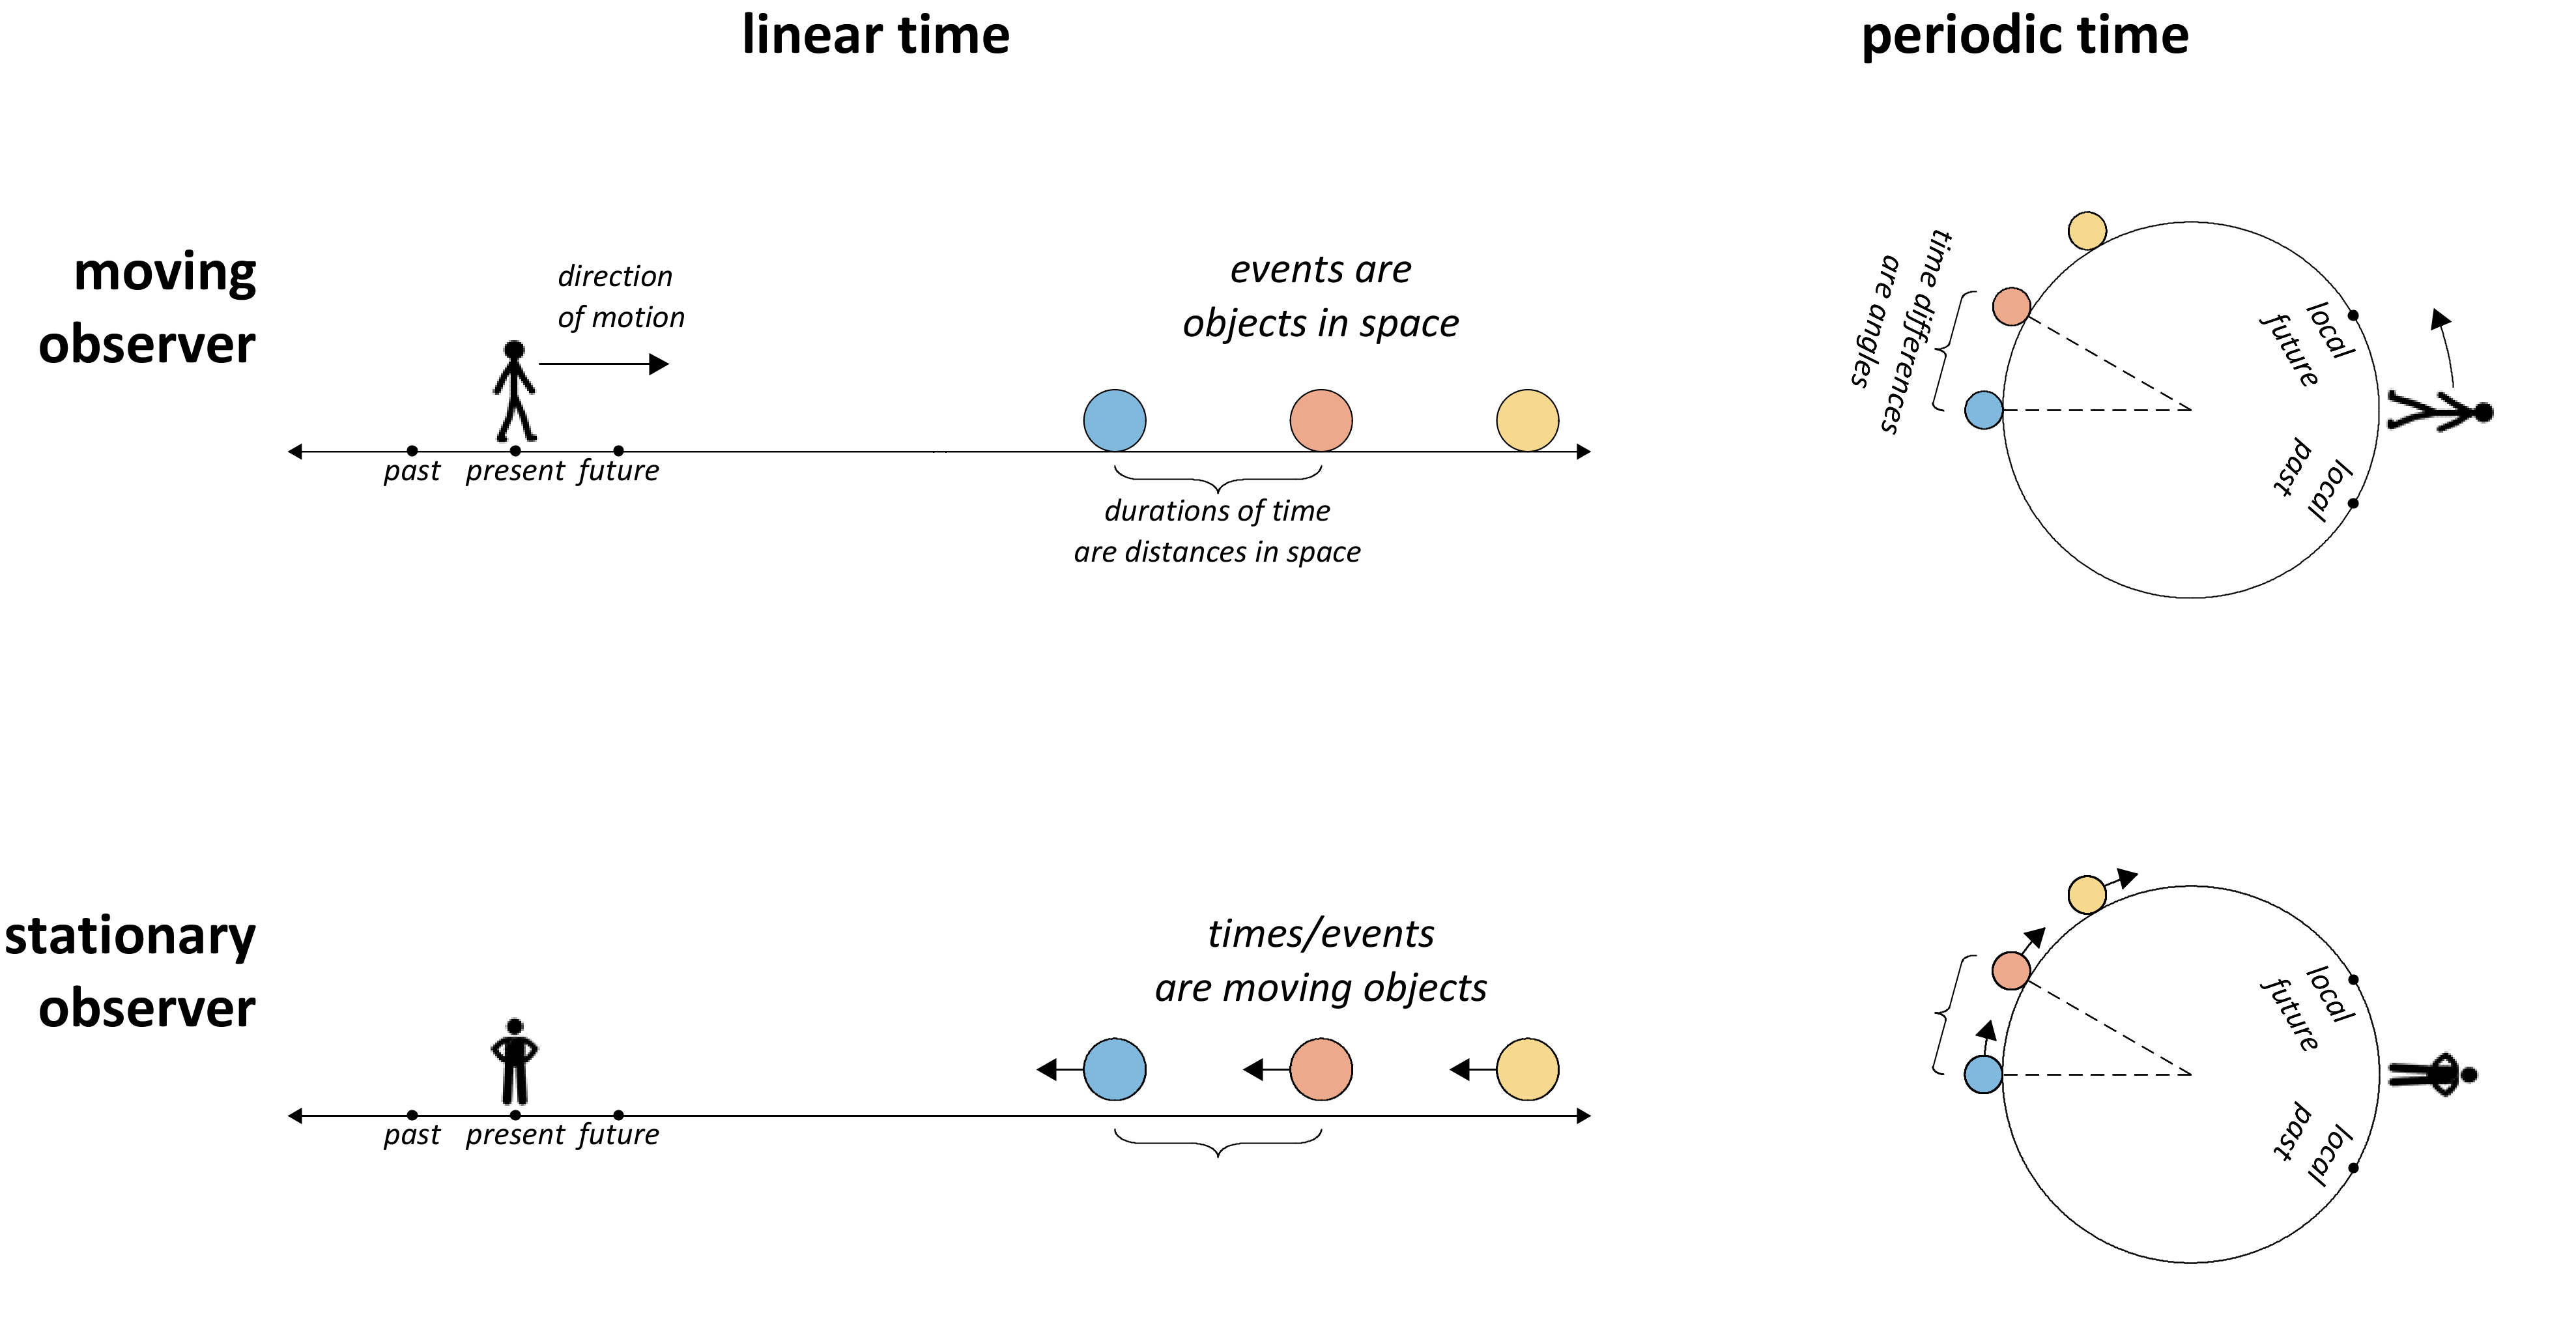
\includegraphics[width=\textwidth]{figures/Tilsen-img38.png}
\caption{Linear and periodic schemas for conceptualizing time.}
\label{fig:3:10}
\end{figure}
 

  In the moving observer linear schema, time is a landscape and an observer moves in a straight line. Events are stationary objects which are located in the landscape (or alternatively, the locations of those objects). In the stationary observer variant, the observer stays put and events are objects which move toward the observer. The moving vs. stationary observer schemas are related by a figure-ground reversal, and we quite often transition between these two schemas in everyday language. Both variants impose temporal asymmetry based on the direction of attention of the observer: the future is \textit{in front of} the observer, because direction of motion and gaze are correlated; likewise, the past is \textit{behind} the observer. These directional mappings give rise to notions of earlier and later, as well as temporal \textit{distance}. 

\subsection{The word order blend}

Words are objects; events in time are objects in space. Via the word order blend, words are objects in a space, and the space represents time. Blending a linear time schema with the object metaphor allows us to conceptualize the temporal ordering of words as a spatial arrangement. The relative order of words corresponds to their relative arrangement (position) in space: temporal order is spatial arrangement. Of course, the technology of writing reinforces this blend: written words are typically arranged in a straight line, with culture-specific variations in orientation and direction. The blend is illustrated below, for both moving- and stationary-observer variations of the schema:

  
\begin{figure}
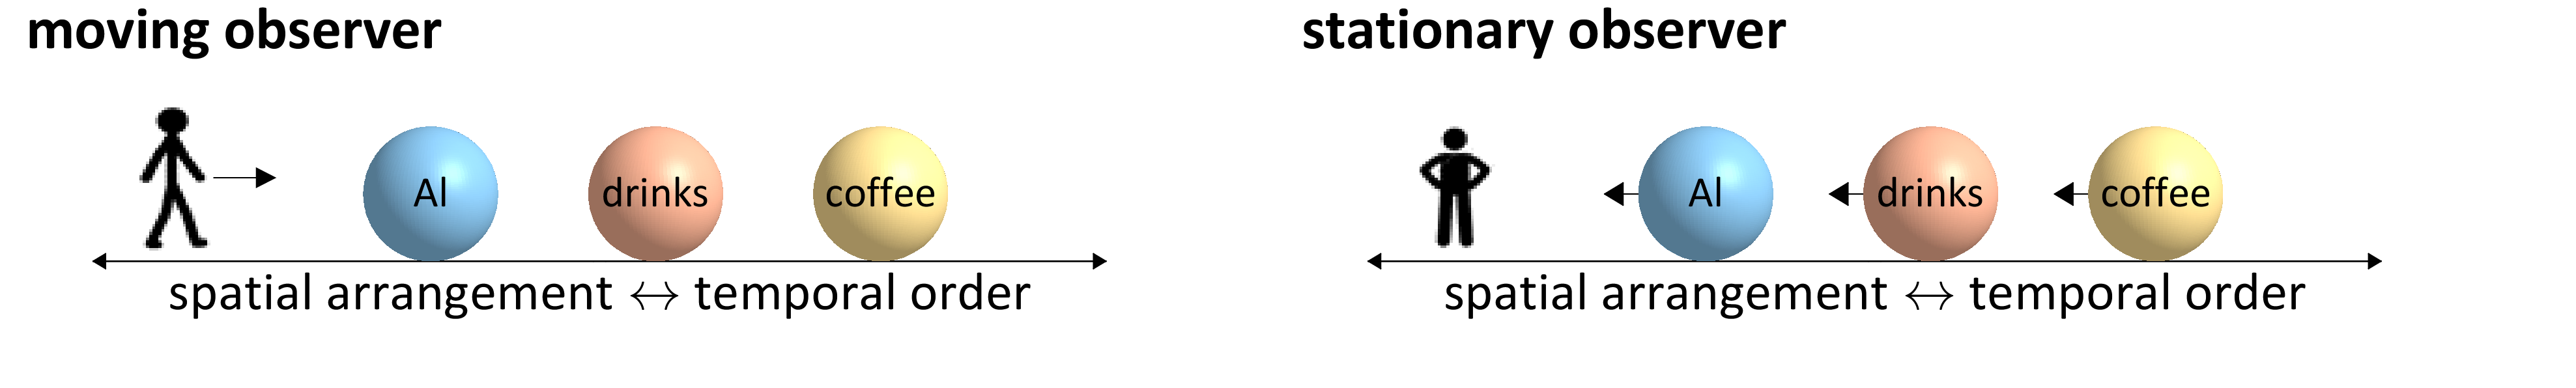
\includegraphics[width=\textwidth]{figures/Tilsen-img39.png}
\caption{The word order blend: temporal order of words is spatial arrangement of objects.}
\label{fig:3:11}
\end{figure}
 

  What role does the word order blend play in conventional syntactic theories? Consider the horizontal spatial arrangement of syntactic objects in (A)-(C) below. Do all of these structures imply the same word order, or do they imply different word orders?

  
\begin{figure}
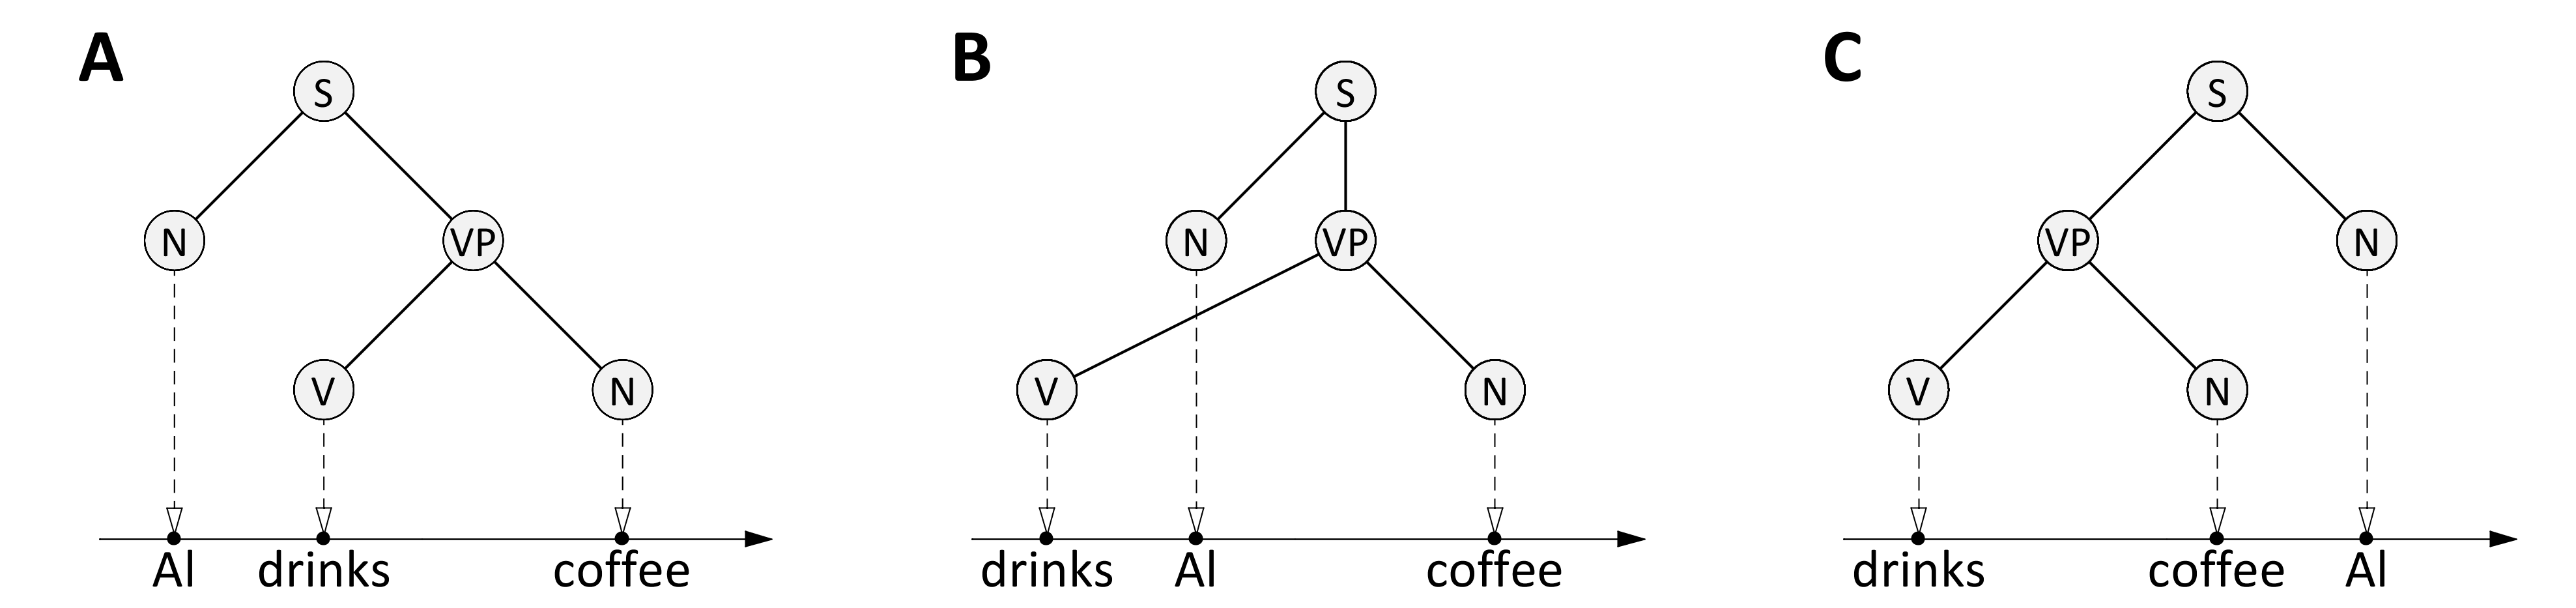
\includegraphics[width=\textwidth]{figures/Tilsen-img40.png}
\caption{Mappings of connected objects structures to word orders.}
\label{fig:3:12}
\end{figure}
 

The structures (A) and (B) are not generally understood as different word orders, but (B) is a somewhat less aesthetically satisfying representation of \textit{Al drinks coffee} than (A), and structures like (B) are less commonly drawn than structures like (A). Structures (A) and (C) can imply different orders, but not necessarily. Indeed, many theoretical frameworks send mixed messages regarding the consequences of spatial arrangement in syntactic trees. Some explicitly reject the blend, but nonetheless habitually conform to it in practice. Lets consider several distinct perspectives:

\begin{enumerate}
\item \textit{The representations are explicitly temporal.}

  In this atypical perspective, representations are held to encode word order. Structures (A) and (C) must be associated with different word orders, and (B) is a bad representation of the utterance \textit{Al drinks coffee}. One can imagine projecting the terminal elements down to a horizontally oriented time axis. This axis need not represent a linear, continuous time, but simply a dimension where temporal order maps to spatial arrangement. The projection process is a simple linearization mechanism. Taking this perspective, (B) does not represent \textit{Al drinks coffee} because \textit{Al} projects down to a location between \textit{drinks} and \textit{coffee}, thereby linearizing the structure as \textit{drinks Al coffee}. (B) may also be considered a problematic representation of \textit{drinks Al coffee} because of line crossing.

\item \textit{The representations are implicitly temporal.}

  In this more common perspective, structures (A) and (C) are associated with different word orders, (B) is equivalent to (A), and (B) is a perfectly fine representation of \textit{Al drinks coffee}. Temporal order is not directly represented by horizontal spatial arrangement of terminal objects, but rather there is a universal algorithm/procedure which maps from local patterns of connection to a local word order. The antisymmetry approach developed in \citet{Kayne1994} is an example of this perspective. As shown below, we can imagine separate, local arrangement schemas are applied to each object based on its local connection structure. The local orderings are uniquely satisfied by a particular temporal order, without requiring a global mapping between horizontal arrangement and temporal order. As shown by the differences in local orderings in (i) and (ii), (A) and (C) are linearized to different word orders.

  
\begin{figure}
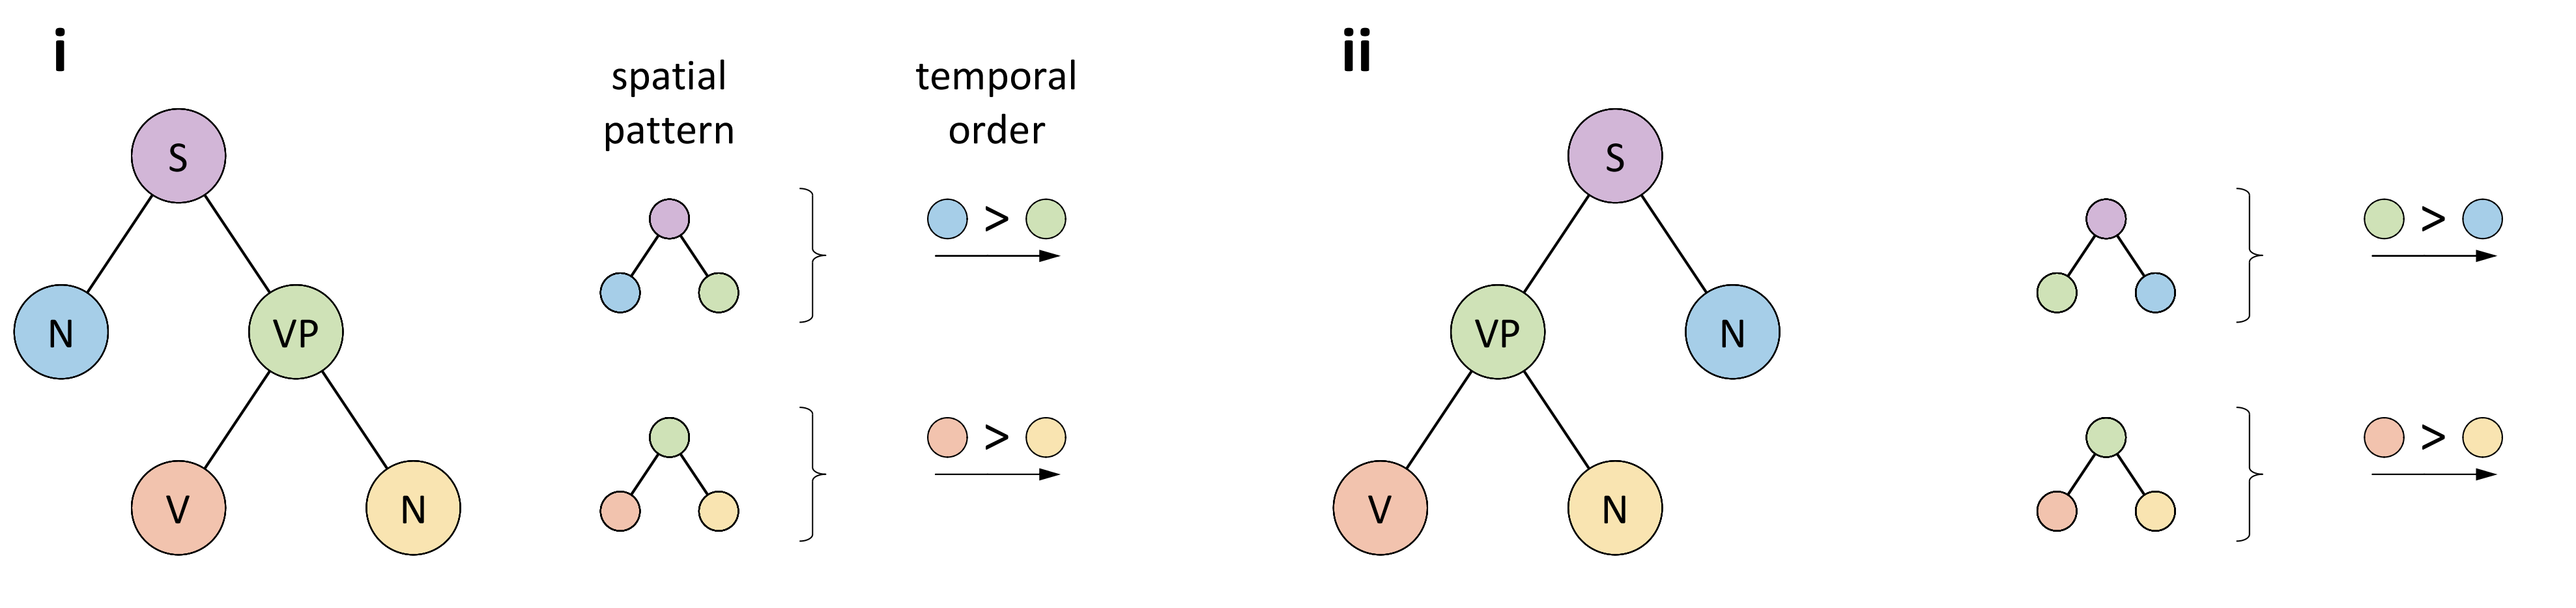
\includegraphics[width=\textwidth]{figures/Tilsen-img41.png}
\caption{Linearization derived from local spatial relations.}
\label{fig:3:13}
\end{figure}
 

\item \textit{The representations are atemporal, linearization produces a temporal representation.}

  The most extreme perspective is that syntactic structures do not encode temporal order in any way, and so (A), (B), and (C) are equivalent. The output of merge operations, for example, is claimed to be an unordered combination of its inputs. The so-called “narrow syntax” does not represent temporal order, and all aspects of order are deferred to an independent linearization mechanism, which can vary across languages. 
\end{enumerate}


\subsection{The hidden temporality of connected object structures}

The atemporal attitude is problematic in two ways, one obvious, one deep. The obvious problem is that a syntactic theory of this sort would seem to have very little to say about word order. Many of the interesting phenomena in language involve the temporal order of words. The deeper and more important problem is that the structure building mechanism \textit{cannot} be independent of the linearization mechanism, all claims to the contrary. Any linearization mechanism must make use of \textit{some} information present in “atemporal” object structures, in order to map them to temporal orders. But if there is some temporal information in the purportedly atemporal structures, then the “atemporal” structures are not \textit{really} “atemporal”—they are covertly temporal. Moreover, this means that the output of the structure building mechanism is predetermined by the linearization mechanism. To see why this is the  case, consider the sequence of structure-building operations shown below.

  
\begin{figure}
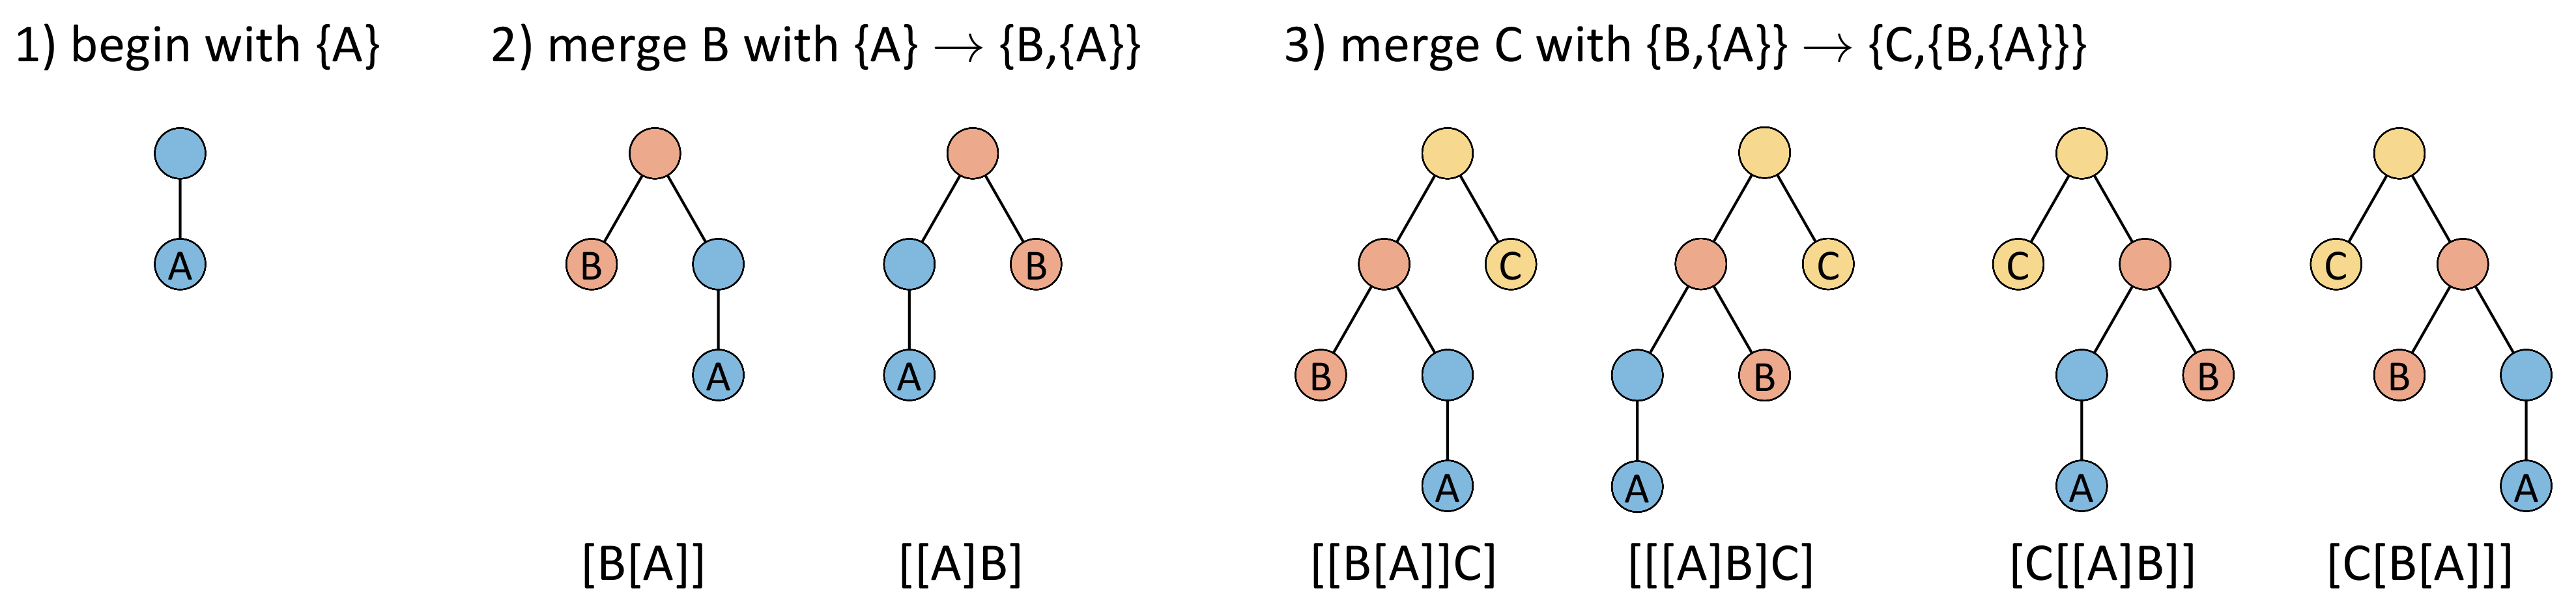
\includegraphics[width=\textwidth]{figures/Tilsen-img42.png}
\caption{Unordered structures which result from a series of merge operations.}
\label{fig:3:14}
\end{figure}
 

  Because \textsc{Merge} produces unordered structures, there are two equivalent representations after the first \textsc{Merge}, and four equivalent representations after the second \textsc{Merge}. These four representations can be linearized to four different orders by vertical projection, as shown below each tree structure. The same four linear orders can also be obtained from a more general linearization procedure, which we describe below.

  The CBA (right-branching) and ABC (left-branching) orders are generated by a simple iterative spell-out algorithm which proceeds up or down in vertical space. To obtain CBA, take the terminal node object from the highest level, spell it out, then move down to the next level and repeat. Observe that all four of the structures in \REF{ex:3:3} generate CBA order with this algorithm. Likewise, the procedure to obtain ABC order from all four structures starts at the lowest level and moves up. Orders BAC and CAB can be produced with somewhat more complicated algorithms which traverse the structure in two different directions. All four algorithms are shown in the {\tablebelow}. 

  \begin{table}
\begin{tabularx}{\textwidth}{XX}
\lsptoprule
CBA & ABC\\
\midrule 
\textsc{Start at highest level}

\textsc{Loop 1}

     \textsc{Find terminal node X on current level}

     \textsc{Spell X out}

     \textsc{Move down one level}

\textsc{Loop 1} & \textsc{Start at lowest level}

\textsc{Loop 1}

     \textsc{Find terminal node X on current level}

     \textsc{Spell X out}

     \textsc{Move up one level}

\textsc{Loop 1}\\
\lsptoprule
BAC & CAB\\
\midrule
\textsc{Start at lowest}\textsc{/}\textsc{most embedded branching node, XP}

\textsc{Loop 1}

      \textsc{Start at highest level in XP}

      \textsc{Loop 2}

         \textsc{Find terminal node X in XP on current level}

         \textsc{Spell X out}

         \textsc{Move down one level}

      \textsc{Loop 2}

      \textsc{Move up from XP to the next branching node}

\textsc{Loop 1} & \textsc{Start at highest}\textsc{/}\textsc{least embedded branching node, XP}

\textsc{Loop 1}

      \textsc{Start at lowest level in XP}

      \textsc{Loop 2}

         \textsc{Find terminal node X in XP on current level}

         \textsc{Spell X out}

         \textsc{Move up one level}

      \textsc{Loop 2}

      \textsc{Move down from XP to next branching node}

\textsc{Loop 1}\\
\lspbottomrule
\end{tabularx}
\caption{Generation of different orders from different linearization algorithms.}\label{tab:3:1}
\end{table}

  Each algorithm generates the same order from all four of the structures in \REF{ex:3:3}. This might suggest that hierarchical structures really could be unordered, or atemporal. But there is something else to notice here. In all cases, the linearization algorithms make use of vertical orientation—information present in the structures—to determine temporal order. Moreover, the procedures require information about which nodes are branching (contain other nodes), and which are terminal (do not contain other nodes). This information is also present in the “narrow” syntactic representation. So in a sense, the information that is required for linearization, information about temporal order, \textit{is} present in the connected object representations. 

  The supposed atemporality of the representations is only a matter of perspective: either we view the structures as atemporal and view orientation and connectivity/containment information as aspects of temporalization; or, we view orientation and connectivity/containment information \textit{as temporal information that is present in the connected object structures}, with linearization making use of this information. 

  More importantly, we can see the order of \textsc{Merge} operations as a source of temporal information. Consider that, from the sequence of \textsc{Merge} operations above, two of the six possible linearizations (i.e. BCA, ACB) of \{C,\{B,\{A\}\}\} cannot be generated without some additional ad hoc mechanism. This is because B merges with A, so A and B have a more direct relation than A and C. Any linearization algorithm of the sort described above must produce an ordering in which A and B are adjacent, and therefore BCA and ACB cannot be obtained.

  The solution to this dilemma is to reorganize the structure itself with “internal \textsc{Merge}”, which is illustrated below. Internal \textsc{Merge} copies an object \REF{ex:3:2}, merges the copied object in the normal way \REF{ex:3:3}, and then ignores the original object \REF{ex:3:4}, which can involve deleting it and/or leaving a trace. The crucial insight is that internal \textsc{Merge} is necessary because the order of \textsc{Merge} operations determines the orientation and connection patterns of syntactic objects, and these in turn constrain linearization. In general, connection patterns determine which spell outs require internal \textsc{Merge}. For any structure resulting from more than one external \textsc{Merge}, there is always some set of spell outs which require internal \textsc{Merge}.

  
\begin{figure}
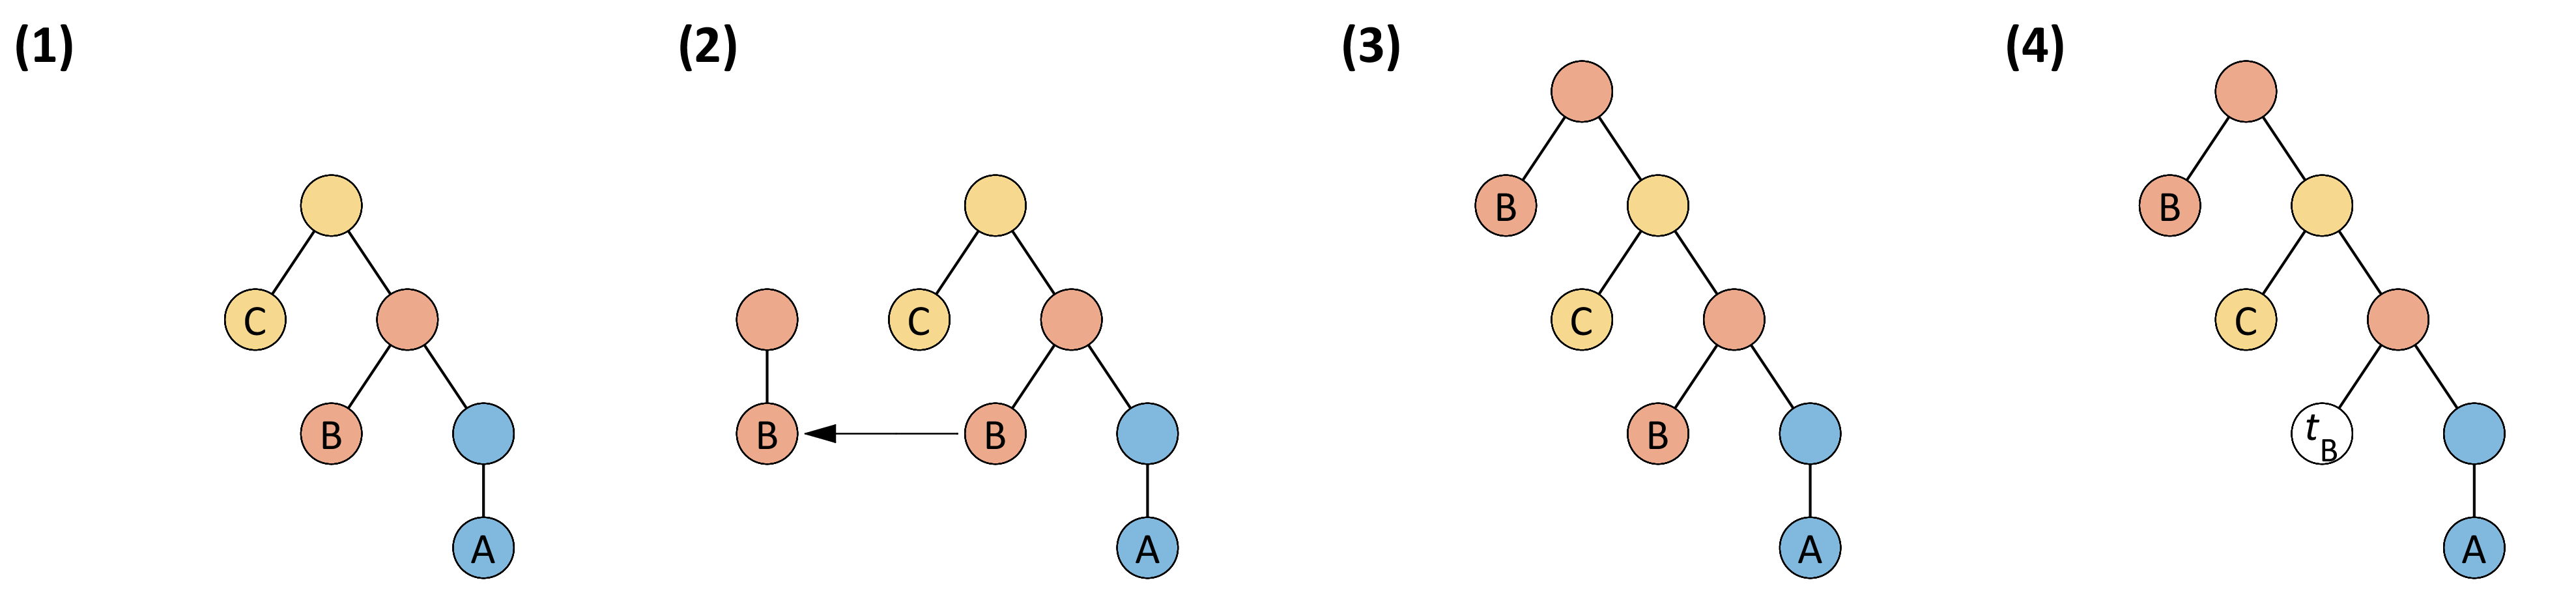
\includegraphics[width=\textwidth]{figures/Tilsen-img43.png}
\caption{Internal merge as copying (2), external merge (3), and deletion leaving a trace (4).}
\label{fig:3:15}
\end{figure}
 

  Whether or not connected object representations are considered “temporal” is a point of view, not an essential characteristic of the representation. The linearization procedure has the property that it requires information regarding dominance (vertical orientation of connection), and so from one point of view, representation of order could be seen as an artefact of linearization, not a feature of the narrow syntax representation. But the \textit{information} needed for the linearization mechanism is present in the narrow representation itself, in the form of dominance relations and connection patterns. This is more obvious when we see that a \textit{structural} change (internal \textsc{Merge}) is necessary to generate some orders from a supposedly “unordered set”. Thus from the alternative point of view, temporal ordering information \textit{is} and \textit{always is} present in the structure. 

  Regardless of which point of view one adopts, relative vertical orientation and \textsc{Merge} necessarily interact. We can see this by comparing the outputs of top-down and bottom-up linearization schemes when applied to root-oriented and tree-oriented structures. As shown below, top-down linearization (i.e. earlier is higher) produces CBA order for a root-oriented structure, and bottom-up linearization (i.e. earlier is lower) produces ABC order for a tree-oriented structure. Thus the temporal information in orientation is implicitly determined by how \textsc{Merge} operates, or vice versa, the operation of \textsc{Merge} is determined by our construal of orientation. The fact that orientational ambiguity renders order ambiguous reinforces this point.

  
\begin{figure}
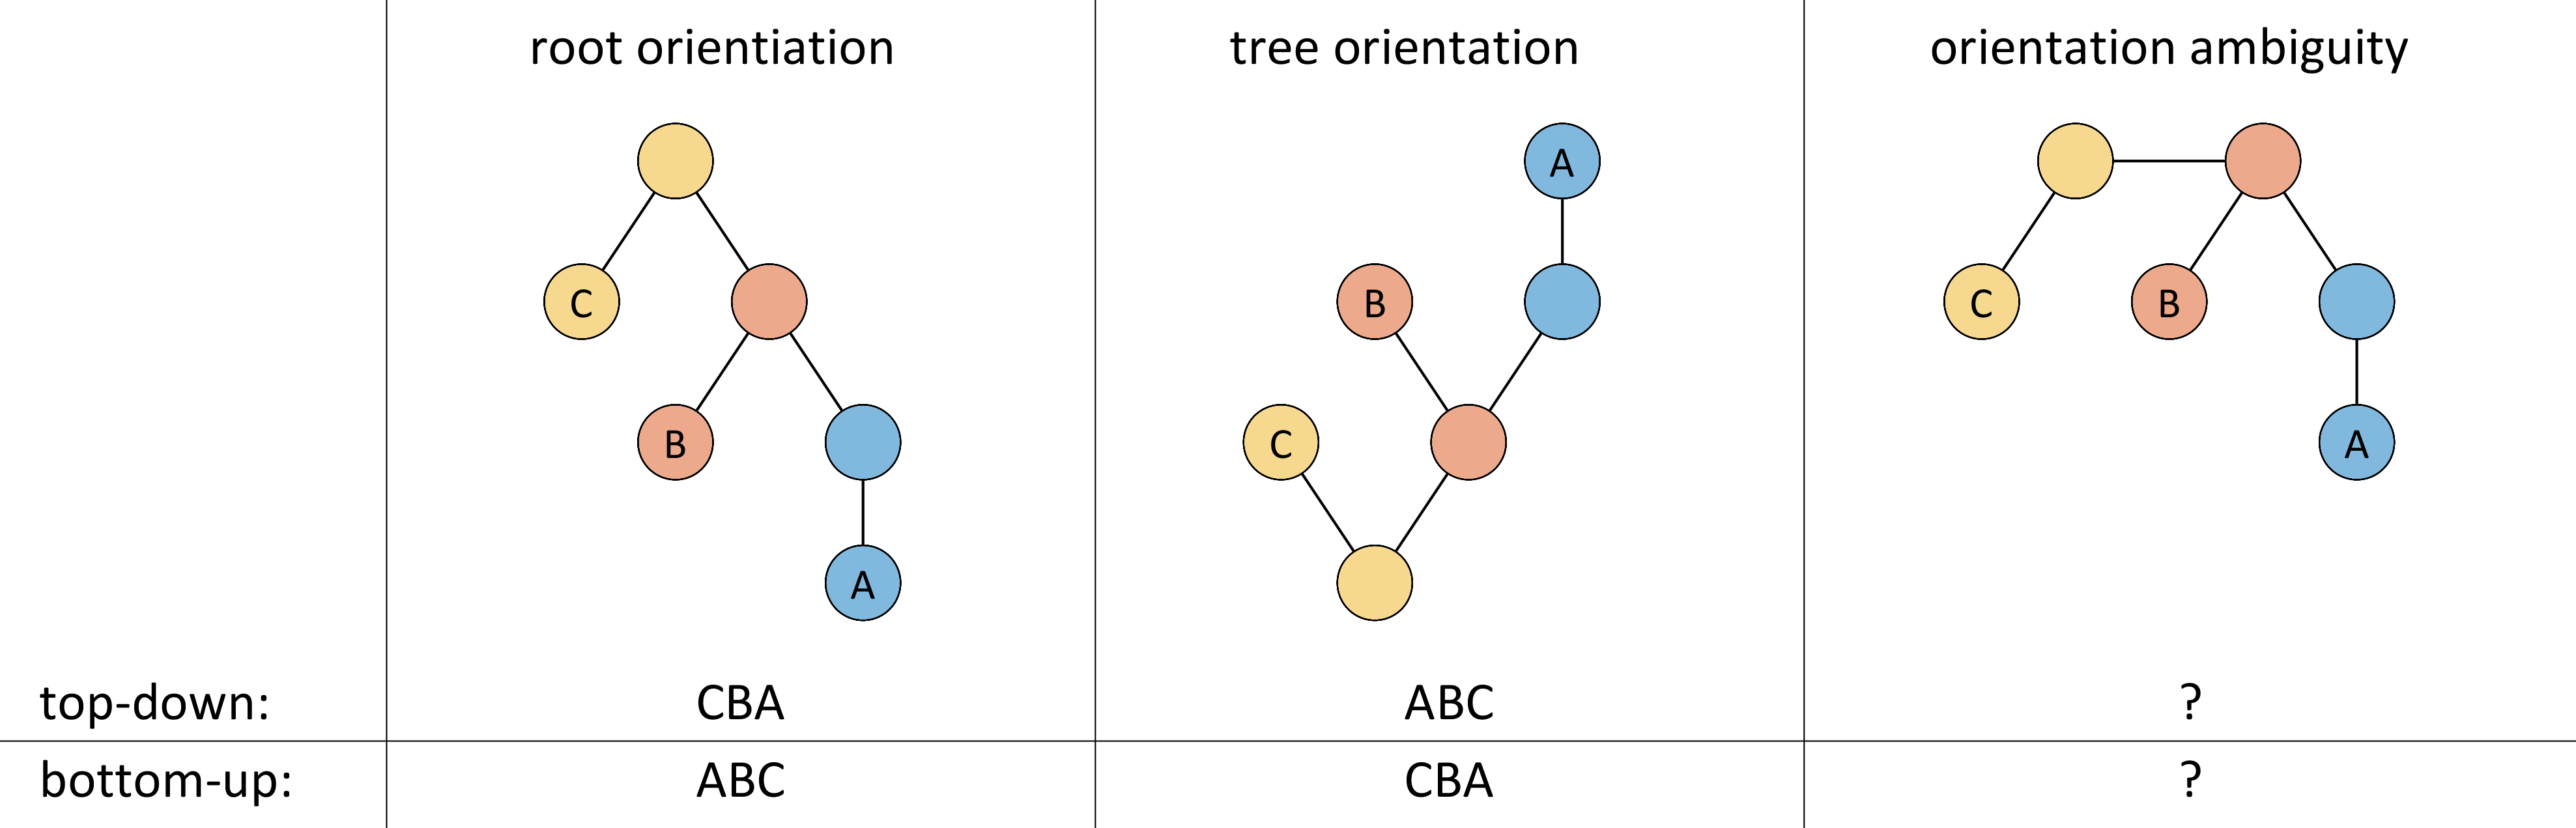
\includegraphics[width=\textwidth]{figures/Tilsen-img44.png}
\caption{Orientation and linearization algorithm determine order.}
\label{fig:3:16}
\end{figure}
 

  Evoking connected object schemas is dangerous because the more we do it, the more we become habituated to conceptualizing language in this way. Nonetheless, the above discussion was necessary because it leads to the conclusion that \textsc{Merge} does not produce atemporal structures—information regarding order is always present. As others have pointed out (e.g. \citealt{Yang1999}), a truly “unordered” representation would be \{A,B,C\}, equivalent to:

  \{A,B,C\} = \{A,C,B\} = \{B,A,C\} = \{B,C,A\} = \{C,A,B\} = \{C,B,A\}

The supposedly “unordered” sets below merely obscure information regarding temporal order:

  \{\{\{A\},B\},C\} = \{C,\{A\},B\}\} = \{\{B,\{A\}\},C\} = \{C,\{B,\{A\}\}\}

Any linearization mechanism, without additional information, requires ordered structure. Concealing temporal order in vertical orientation and connection patterns, or in containment and embedding patterns, does not eliminate temporal order; it merely makes the temporal information more difficult to identify. 

\subsection{Essential vs. effective time}

The output of linearization is conventionally conceptualized with a linear time schema. This linear time schema is very general, underlying the conception of speech as a \textit{string} of words (moving observer) or as a flow/stream of words (stationary observer). What makes these conceptions of time “linear”?  The linearity is not simply the property that time is mapped to a \textit{straight line} or a \textit{straight trajectory}. The fundamental character of linearity is that any given segment of space/time is equivalent to any other one, no matter where/when those segments are located/occur, as long as those segments are the same length/duration. 

  Linearity implies a straight line relation between \textit{essential time} and \textit{effective time}. Effective time is an analytical tool, a made-up dimension of time, viewed as orthogonal to essential time. Essential time is a dimension of time that corresponds to our folk understanding \textit{what} time \textit{is}, i.e. our intuitive assumptions that time is absolute, progresses uniformly, and is independent of the observer.

  
\begin{figure}
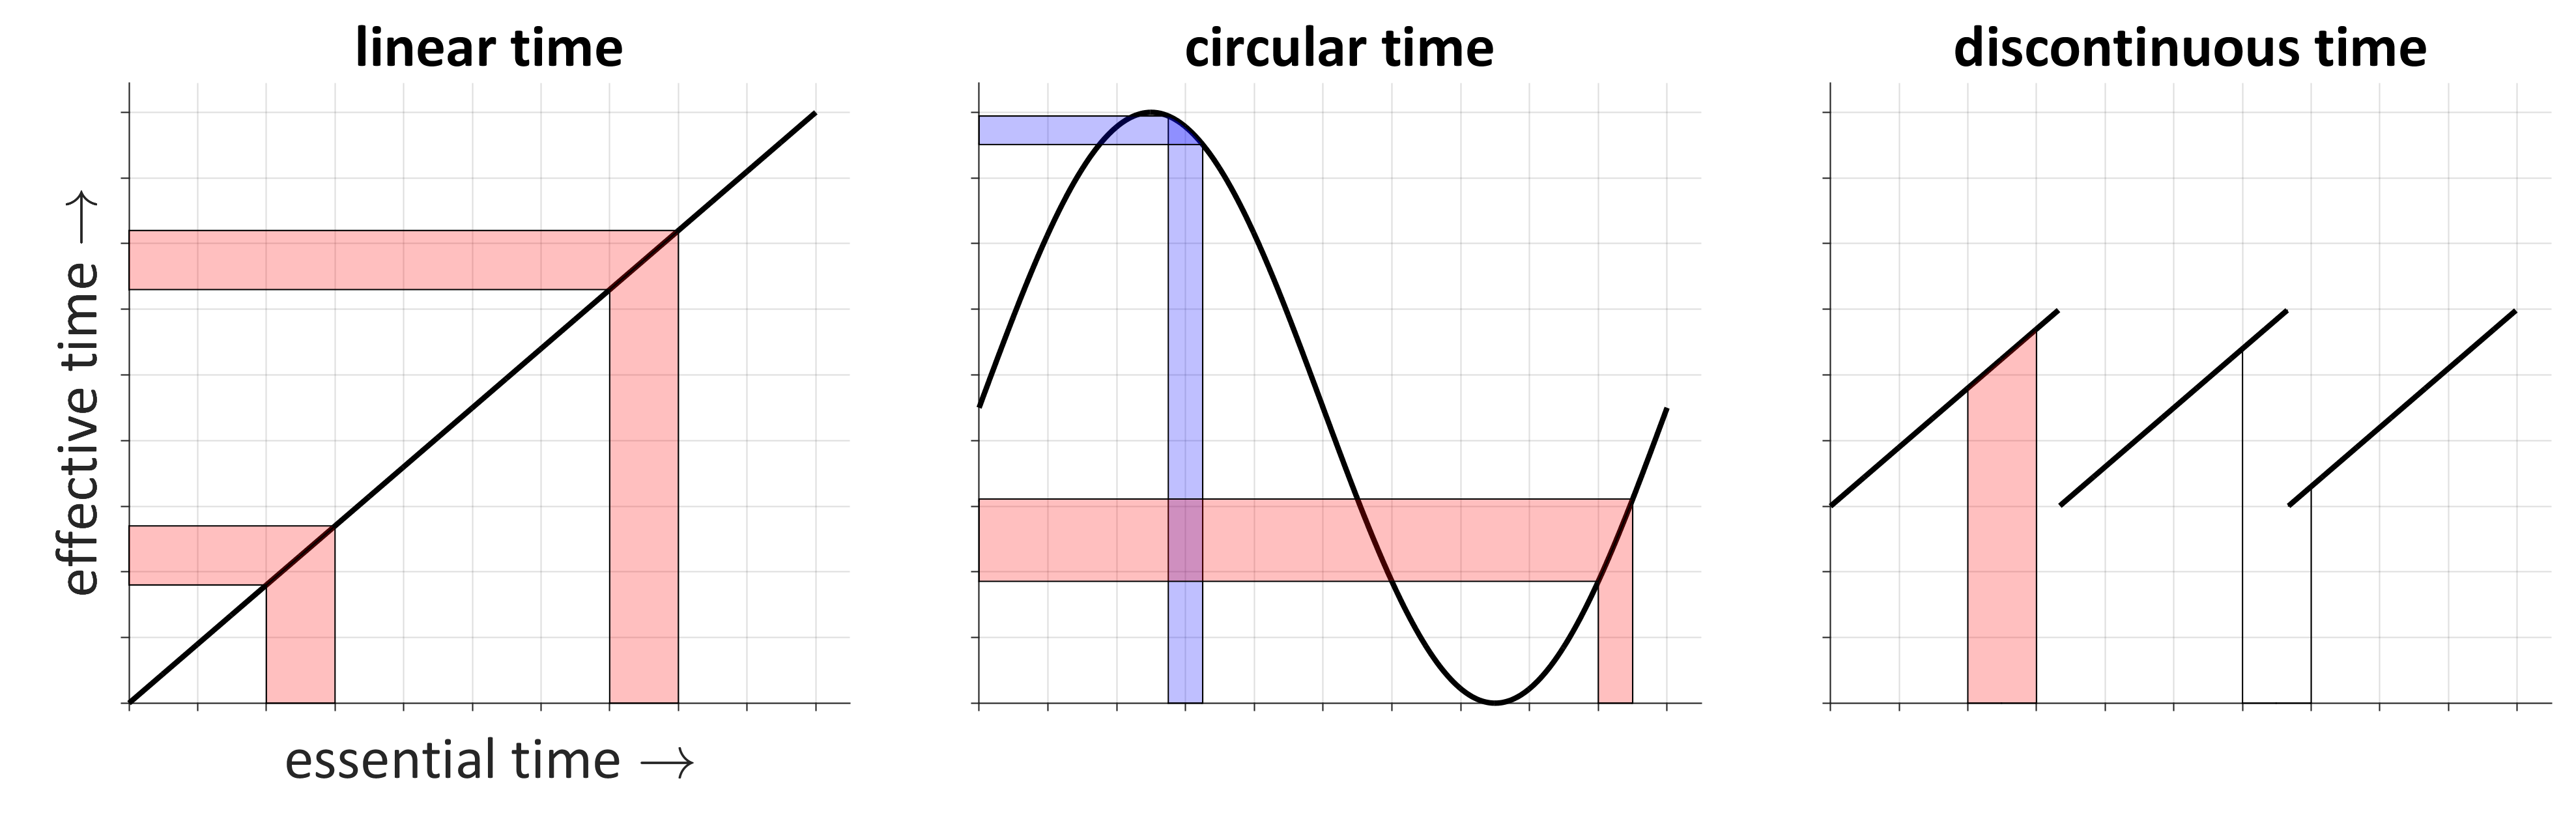
\includegraphics[width=\textwidth]{figures/Tilsen-img45.png}
\caption{Differences between linear, circular, and discontinuous time illustrated as relations between essential time and effective time.}
\label{fig:3:17}
\end{figure}
 

  Effective time is associated with a measure of a quantity that accumulates as essential time progresses. Consider for example an effective time quantity which accumulates at a constant, non-zero rate. For an interval of essential time of a given duration, the amount of the quantity accumulated during the given interval will be the same, regardless of \textit{when} the interval occurs. In linear time, the function relating essential time to the effective time quantity has a constant first derivative and all higher-order derivatives are zero. For example, linear time is appropriate for describing a person walking at a constant pace. If the number of steps taken is the accumulating quantity, and thus the measure of effective time, then the functional relation between essential time and effective time is a straight line. The choice of the quantity to measure is arbitrary. What is crucial is that we evoke a schema in which temporal distance maps to spatial distance, and in which this occurs in a \textit{linear} manner.

\subsection{Periodic time}

Another useful conception of time is one in which the effective time quantity is a periodic function of  essential time. This enables us to equate any moment with a set of past and future moments, leading to a picture of a closed-loop time axis, and hence phase angle, θ. Periodic time is useful in the o/el framework because variation in the order parameters of conceptual and syntactic populations is conjectured to have an oscillatory component.

  
\begin{figure}
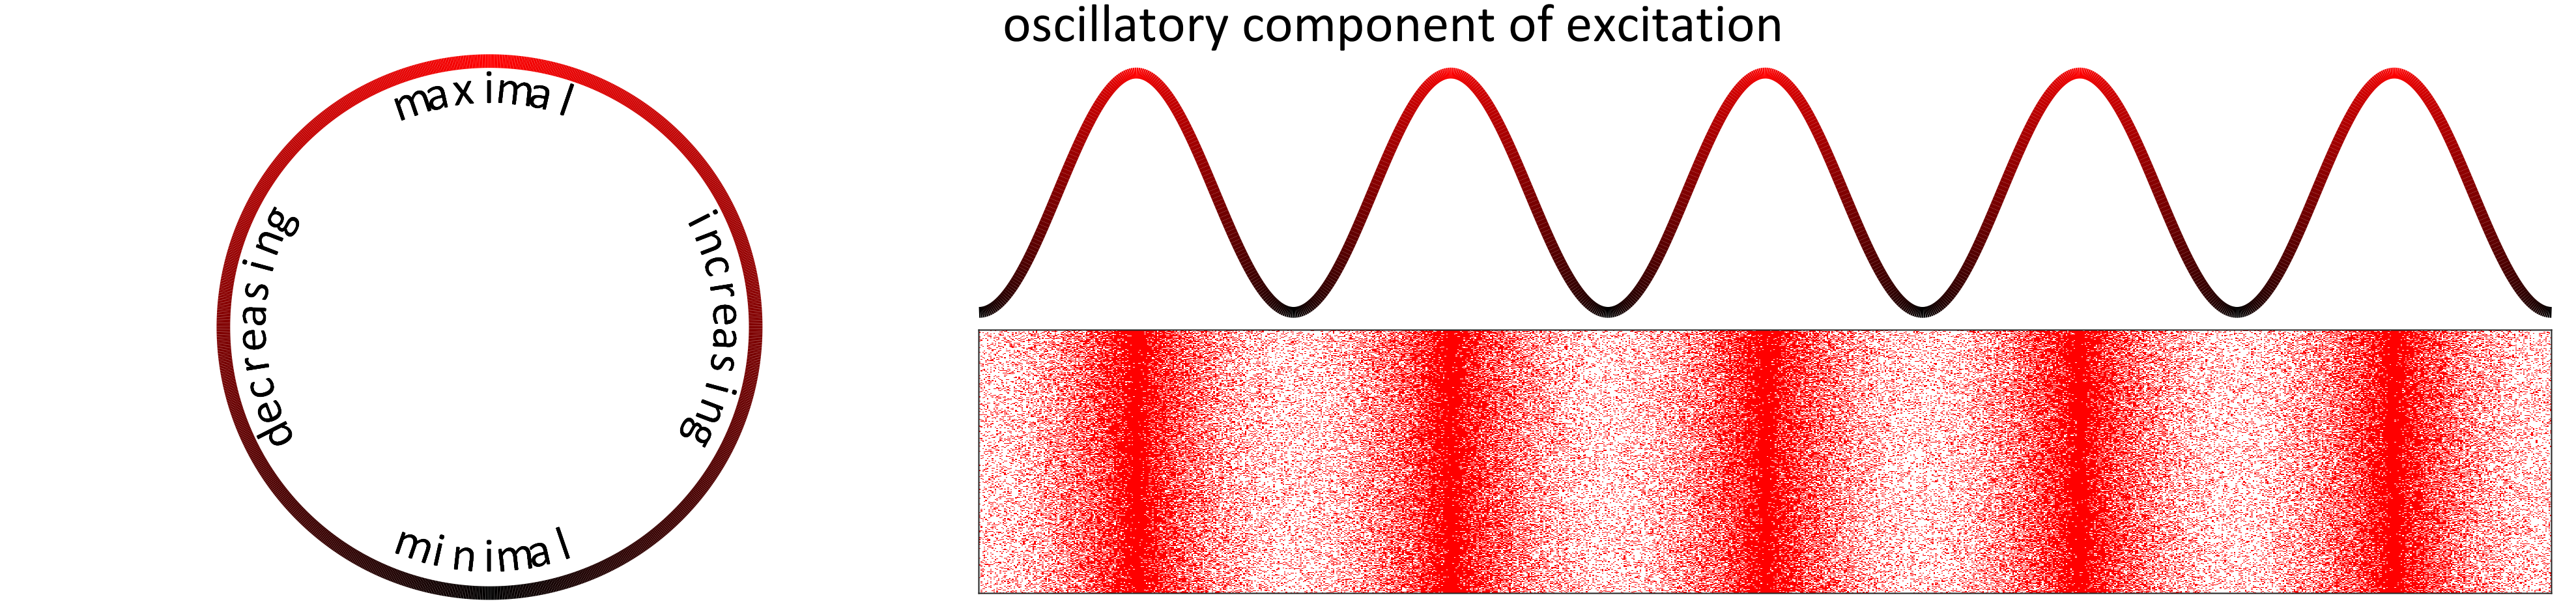
\includegraphics[width=\textwidth]{figures/Tilsen-img46.png}
\caption{Periodic variation in the integrated spike rate of a population can be mapped to phases of an oscillatory system.}
\label{fig:3:18}
\end{figure}
 

  From a macroscopic perspective, the effective time quantity of a system is θ(t). On the microscale, we can construct the oscillatory component of the order parameter to be \textit{x}\textsubscript{osc} = α sin θ and so its derivative is α cos θ. If we define the reference phase as θ = 0, then θ = 0 is when \textit{x} is maximally increasing, θ = π/2 is when \textit{x} is maximal, θ = π is when \textit{x} is maximally decreasing, and θ = 3π/2 is when \textit{x} is minimal. However, this particular mapping of θ to population microstates is an arbitrary consequence of our choice of reference phase and counterclockwise direction of motion. There is no reason, other than convenience, not to reformulate the relation with 12:00 as a reference or as a clockwise motion in Cartesian coordinates. We have also assumed for simplicity that the oscillations are approximately harmonic, but one can imagine a number of alternatives as below. What is crucial is not the precise form of the oscillation, but rather its periodic nature, which entails symmetry under rotations of 2π radians. Accordingly, there is a discrete time-translation symmetry in essential time, under integer multiples of translations of T = \textit{f}\textsuperscript{{}-1} = 2$\pi \omega $\textsuperscript{{}-1}, where \textit{f} is the frequency in cycles/sec, ω is angular frequency in radians/sec, and T is the cycle period.

  
\begin{figure}
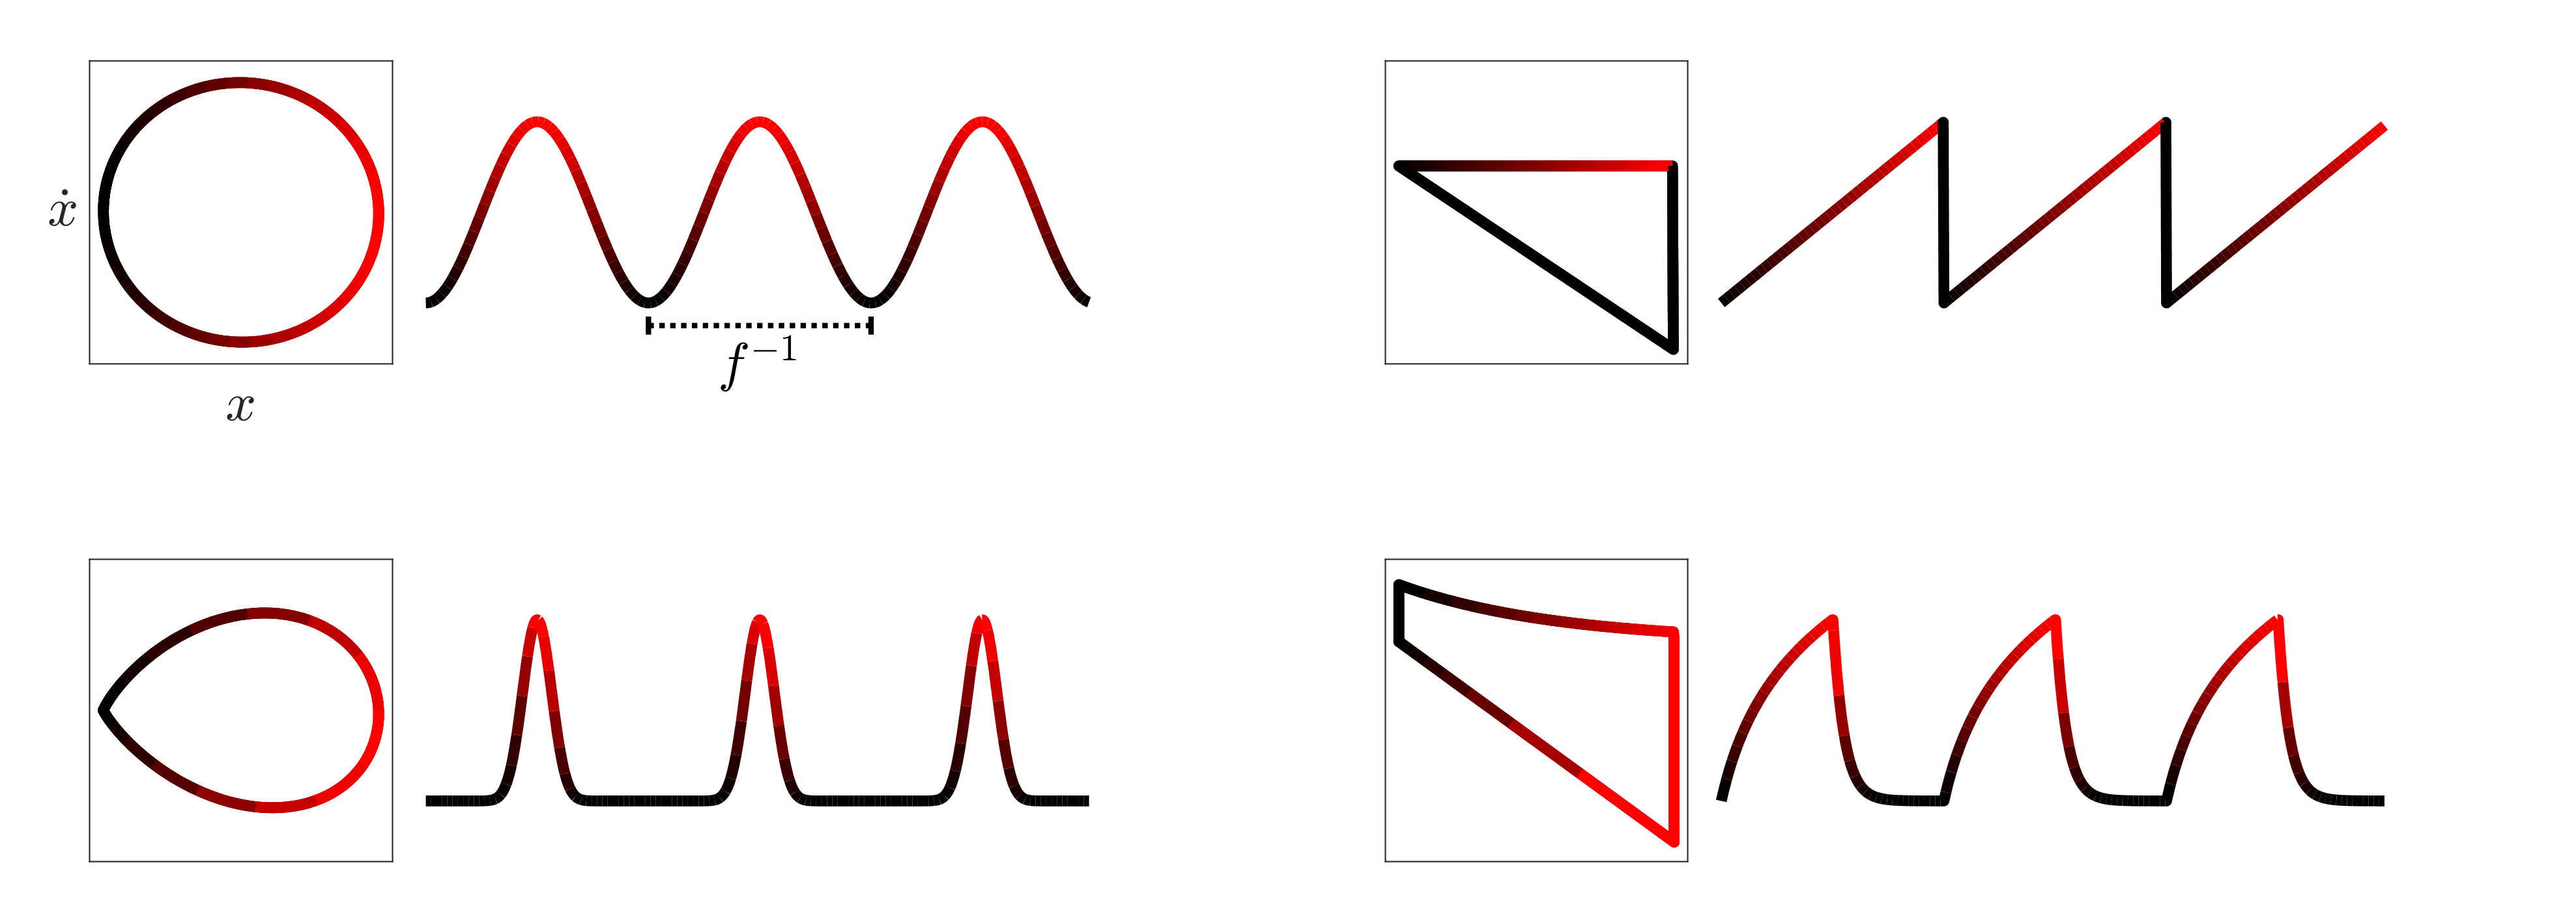
\includegraphics[width=\textwidth]{figures/Tilsen-img47.png}
\caption{Non-harmonic periodic trajectories.}
\label{fig:3:19}
\end{figure}
 

  Because of its discrete time translation symmetry, periodic time has only local notions of past, present, and future. There is no global past/future in a periodic time schema because the time axis, though unbounded, is finite. A moving observer, who is at some location (θ), will eventually return to that same location. There is also no inherent way to decide which location is visited first: the moving observer can only decide that some particular phases are visited \textit{relatively} before or after others, where the qualifier \textit{relatively} expresses the locality of the relation, which must be less than (2\textit{f})\textsuperscript{{}-1}, i.e. less than half the period of the cycle. Likewise, a stationary observer will experience the same sequence of events forever, but has no inherent way to decide which event begins the sequence. Hence circular time has no global conception of temporal order, only a local one. 

  Why is the absence of a global past and present important? The principle of relational meaning holds that relational meaning experiences are stable φ patterns. Periodic time provides a more natural description of this condition, since φ is invariant despite change in θ. Moreover, in a periodic time schema, the minimal and maximal φ differences between systems are 0 and ±π, and these are the two φ configurations we are most interested in. Thinking of such relations in terms of linear time obscures this form of temporal invariance. For example, variation in arousal and other surroundings mechanisms may induce variation in the absolute timing of spike rate maxima of populations, i.e. variation in Δt. Such variation is illustrated in the {\figurebelow}, which shows waveforms of different frequencies. However, by factoring out such variation with the relation 2π\textit{f}Δt = $\omega \Delta $t = φ, we can ignore irrelevant differences in absolute timing and recognize a fundamental invariance in relative phase. The frequency \textit{f} can thus be viewed as a normalization device, a tool for factoring out variation we are not interested in.

  
\begin{figure}
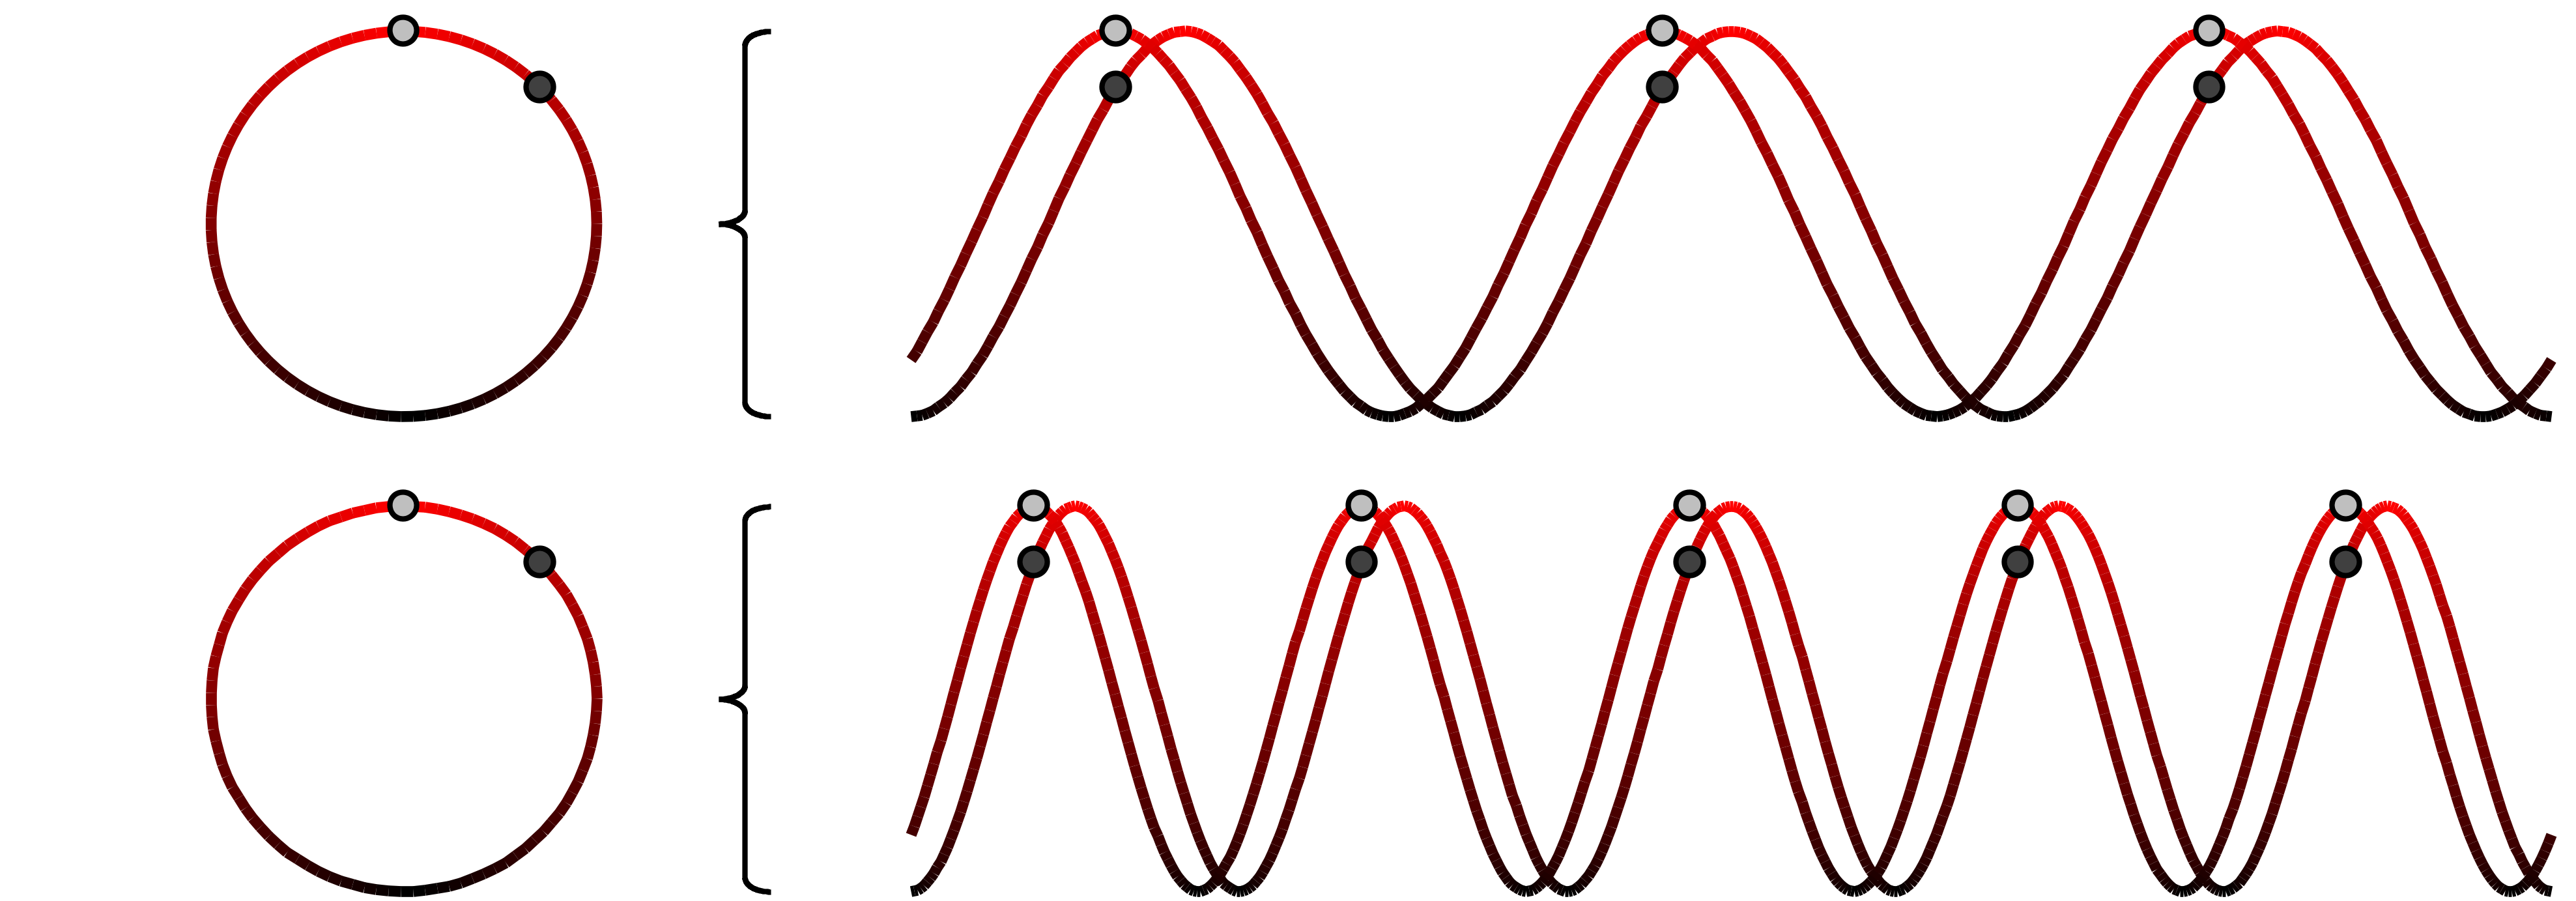
\includegraphics[width=\textwidth]{figures/Tilsen-img48.png}
\caption{The relative phase of frequency-locked oscillating systems does not depend on the frequency of oscillation.}
\label{fig:3:20}
\end{figure}
 

  Periodic time also allows us to see all meaning experiences as a form of symmetry breaking. Consider that an inactive population—which gives rise to no meaning experience—has continuous time reversal and translation symmetries (action potentials are uncorrelated). The emergence of a collective oscillation breaks these symmetries, but preserves a discrete/periodic translational symmetry.

\subsection{Discontinuous time}

The discontinuous time schema is a blend of a discontinuity schema with linear time. In continuous linear time, the linearity property is \textit{global}, applying at all locations in time/space. Moreover, the time/space line is continuous and infinite, extends forever in both directions, and there are no locations which are not “connected” to all other locations. In contrast, these properties do not hold for discontinuous time. By imposing a \textit{discontinuity schema} on linear time, discontinuous time separates time/space into pieces (epochs) which are disconnected from each other. Thus we expect some effective time quantities to change discontinuously “between” epochs. This is useful for conceptualizing the hypothesized reorganization mappings of the excitation operator Ê, which are so fast that they appear discontinuous on the scale in which e configurations remain stable. In a sense, discontinuous time helps us avoid worrying too much about the internal dynamics of e configuration reorganizations. Instead, we focus on stable e configurations within epochs.

  
\begin{figure}
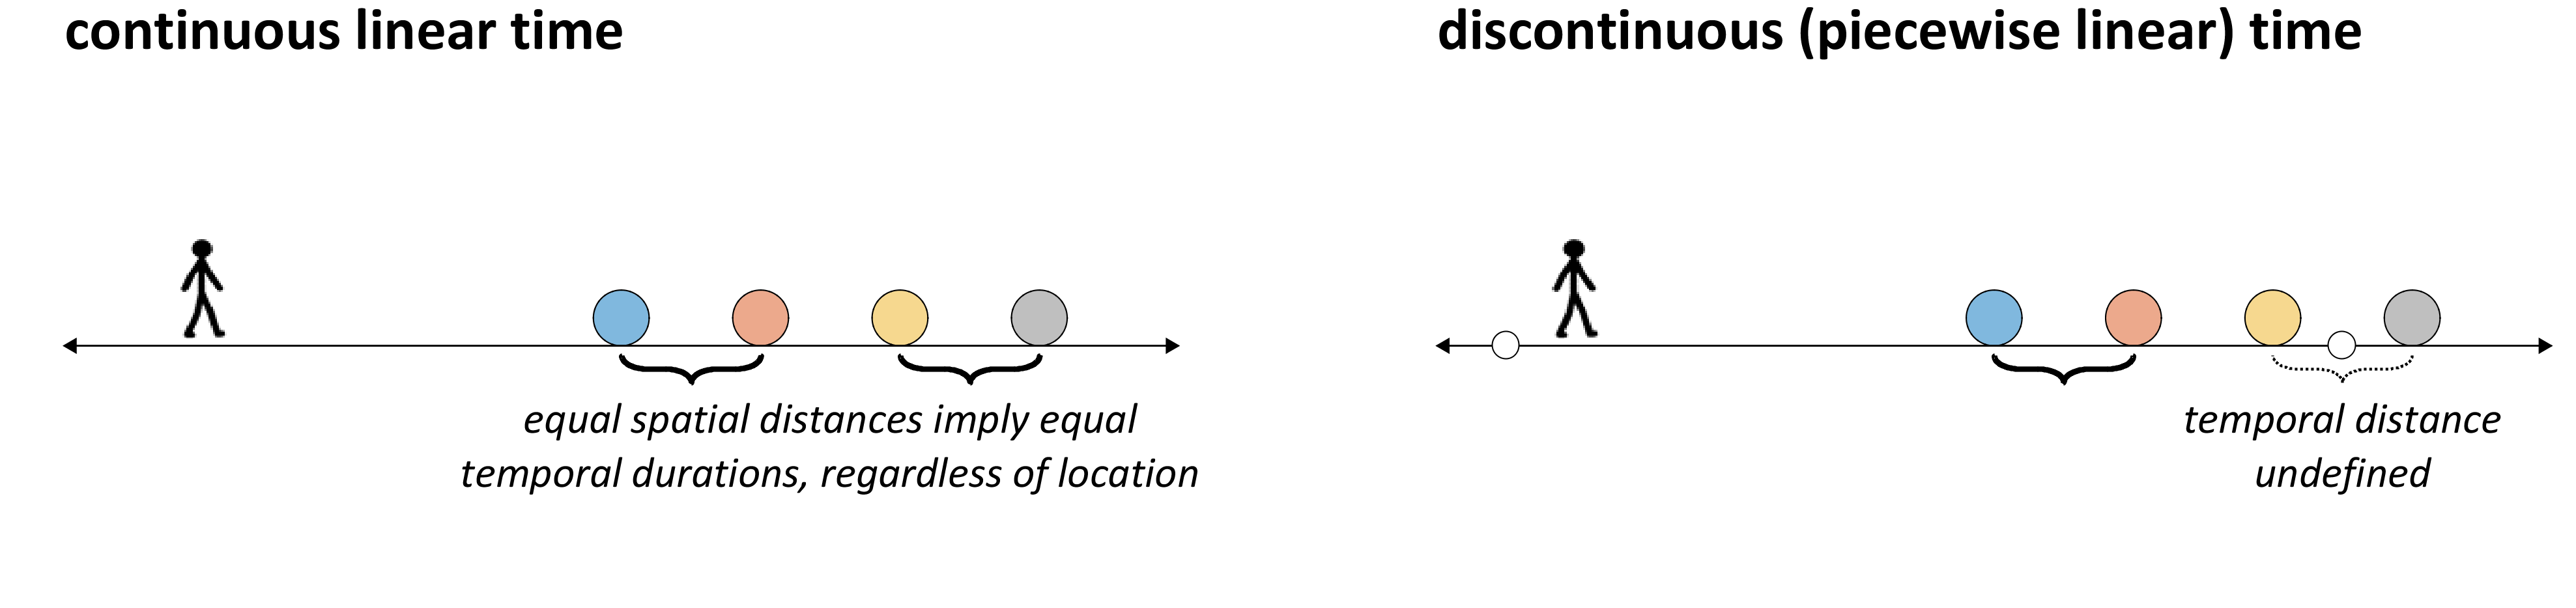
\includegraphics[width=\textwidth]{figures/Tilsen-img49.png}
\caption{Comparison of continuous and discontinuous time schemas. Some temporal distances between events are undefined in discontiuous time.}
\label{fig:3:21}
\end{figure}
 

  The time-integral of the excitation state variable (\textit{e}) is an effective time quantity which exhibits discontinuities in its first derivative between stable e-epochs. Recall that the canonical e-reorganization involves demotion of a selected system and promotion of other excited systems. As shown below, the effective time quantity \textit{e} changes abruptly in the transitions between epochs, and is constant within them. Consequently there is an elbow (discontinuity in first derivative) in the time-integral of \textit{e}. This is particularly relevant when we consider that feedback mechanisms influence when reorganizations occur. Feedback may be correlated with the integral of selection-level excitation; when the integral of selection-level excitation reaches a threshold, a reorganization occurs.

  
\begin{figure}
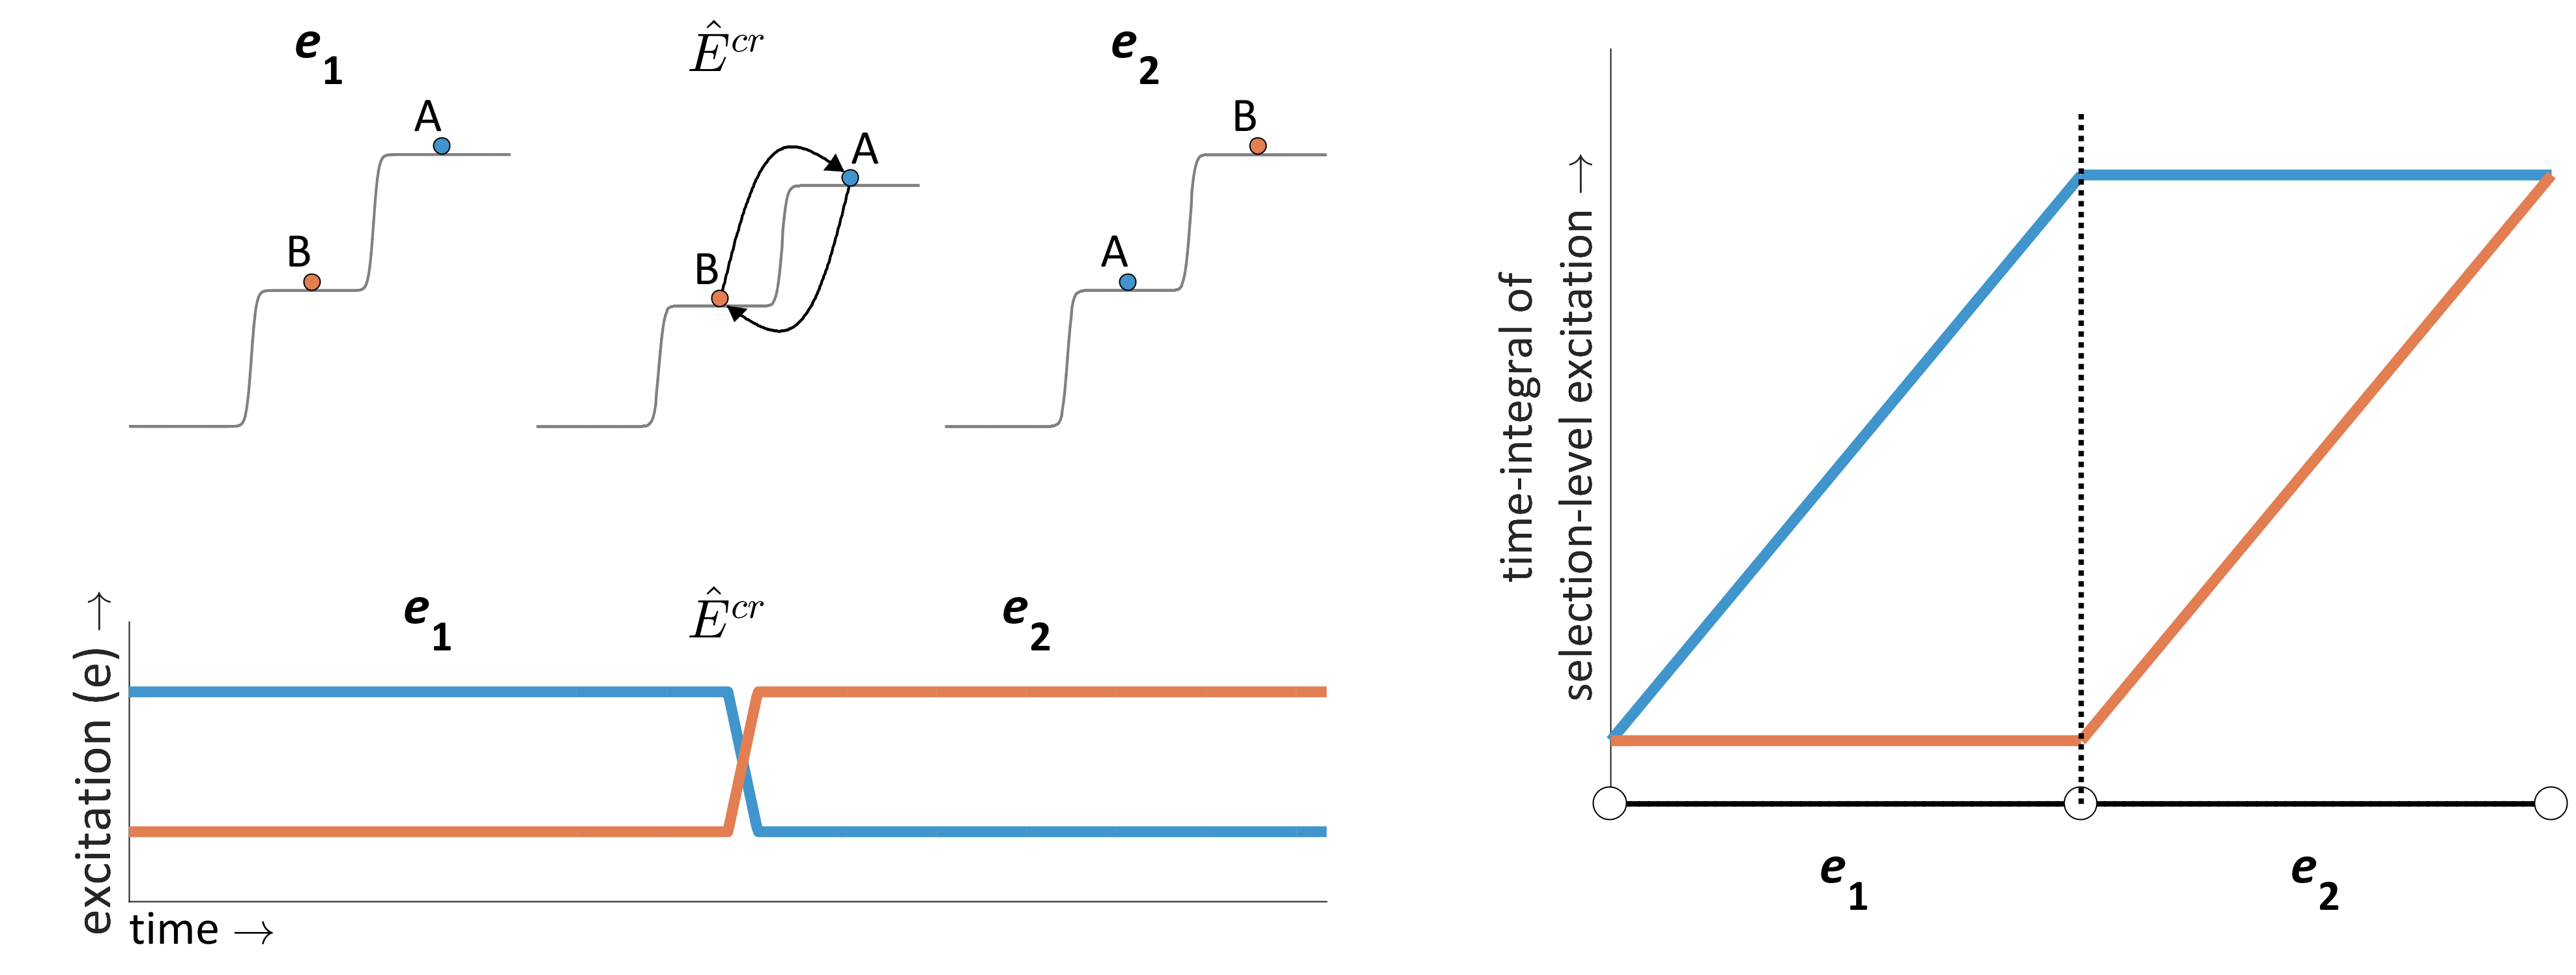
\includegraphics[width=\textwidth]{figures/Tilsen-img50.png}
\caption{Discontinuous time is well-suited for understanding the dynamics of excitation.}
\label{fig:3:22}
\end{figure}
 

  Another reason the discontinuous time schema is useful is that we cannot readily blend it with the words-are-objects metaphor. The object metaphor evokes a static, time-invariant structure that persists throughout an utterance. The discontinuous time schema is antithetical to that sort of conception, because it does not gel with persistence across multiple e-epochs. 

  Our analyses of linguistic patterns can be improved by conceptualizing time as multiform: different conceptions of time are useful for different phenomena on different scales. This is a consequence of the inherent complexity of language: linguistic patterns arise from interactions between systems on a wide range of spatial and temporal scales; to impose a single temporal schema on a given analysis, or even worse to ignore time altogether, is a counterproductive oversimplification. 

